%%%%%%%%%%%%%%%%%%%%%%%%%%%%%%%%%%%%%%%%%%%%%%%%%%%%%%%%%%%%%%%%%%%%%%%
%% August 7, 2015
%%
%% JLAB-THY-15-xxxx
%%%%%%%%%%%%%%%%%%%%%%%%%%%%%%%%%%%%%%%%%%%%%%%%%%%%%%%%%%%%%%%%%%%%%%%
\documentclass[aps,prd,amsmath,preprint]{revtex4}

% \voffset 1cm

\usepackage[utf8]{inputenc}
\usepackage{enumerate}
\usepackage{amsmath,amssymb}
\usepackage{bm}
\usepackage{amscd}            % for extensible arrows (e.g., limits)
% \usepackage{epsfig}
\usepackage{graphicx}
\usepackage{hhline,multirow}  % for nicer tables
\usepackage{dcolumn}          % Align table columns on decimal point
\usepackage{url}              % for URL addresses
\usepackage[colorlinks=true,linkcolor=blue]{hyperref}
\usepackage{color}

\newcommand{\mc}{\multicolumn}
\newcommand{\s}{\hspace*{.2cm}}
\newcommand{\tik}{\checkmark}

\preprint{JLAB-THY-15-xxxx}

\begin{document}

\title{Constraints on large-$x$ parton distributions from new \\
	weak boson production and deep-inelastic scattering data}

\author{A.~Accardi$^{1,2}$,
	L.~T.~Brady$^{2,3}$,
	P.~J.~Ehlers$^{2,4}$,
	C.~E.~Keppel$^2$,
	W.~Melnitchouk$^2$
	J.~F.~Owens$^5$,
	Nobuo~Sato$^2$}

\affiliation{
$^1$\mbox{Hampton University, Hampton, Virginia 23668} \\
$^2$\mbox{Jefferson Lab, Newport News, Virginia 23606} \\
$^3$\mbox{University of California, Santa Barbara, California 93106, USA} \\
$^4$\mbox{University of Washington, Seattle, Washington 98195, USA} \\
$^5$\mbox{Florida State University, Tallahassee, Florida 32306, USA} \\
{\bf CTEQ-Jefferson Lab (CJ) Collaboration}\\
}


\date{\today}

\begin{abstract}
We present a new set of leading twist parton distribution functions
(PDFs), which take advantage of developments in the theoretical
treatment of nuclear corrections as well as new data.
The analysis includes for the first time data on the free neutron
structure function from the BONuS experiment at Jefferson Lab,
and new $W$-boson asymmetry data from Fermilab, both of which
significantly reduce the uncertainty on the $d/u$ ratio at large
values of $x$.
We also review evidence for a sign change in $\bar d-\bar u$ at
large $x$ that has been claimed in recent phenomenological analyses.
\end{abstract}

\maketitle


%%%%%%%%%%%%%%%%%%%%%%%%%%%%%%%%%%%%%%%%%%%%%%%%%%%%%%%%%%%%%%%%%%%%%%%%%
\section{Introduction}
\label{sec:intro}

... general intro ...

... what is new since CJ12 ...

$\bullet$
more complete/consistent/systematic treatment of nuclear corrections
esp. nucleon off-shell corrections

$\bullet$
impact of new $W$-boson asymmetry data on $d/u$ ratio

$\bullet$
inclusion of JLab (BONuS) data

$\bullet$
analysis of $\bar d - \bar u$ at large $x$

$\bullet$
S-ACOT scheme for heavy quarks

$\bullet$
LO fit

$\bullet$
$\alpha_s$ treatment



... In Sec.~\ref{sec:thy} we ...


% In the following section we describe the methodology involved in the
% fits, including the choices of data sets, the parametrizations used,
% and the treatment of nuclear and finite-$Q^2$ corrections.  We also
% discuss the treatment of the experimental errors and the resulting
% error PDF sets.  In Sec.~\ref{sec:results} we present an overview of
% the CJ12 PDF results, and compare these with results from other global
% fits.  Finally, in Sec.~\ref{sec:conclusion} we make some concluding
% remarks and outline plans for future work.  An appendix is provided
% which contains the initial parameter values for each of the PDF sets.


%%%%%%%%%%%%%%%%%%%%%%%%%%%%%%%%%%%%%%%%%%%%%%%%%%%%%%%%%%%%%%%%%%%%%%%%%
\section{Theoretical foundations}
\label{sec:thy}

In this section we present the theoretical framework that is used for
the CJ15 analysis.


% .......................................................................
\subsection{PDF parametrizations}
\label{ssec:parametrizations}

{\color{blue}
...[OLD TEXT]...

For the parametrization of the PDFs at the input scale $Q_0^2$,
a common form has been adopted for all parton species $f$,
%
\begin{equation}
xf(x,Q_0^2) = a_0 x^{a_1} (1-x)^{a_2} (1 + a_3 \sqrt{x} + a_4 x).
\label{eq:param}
\end{equation}   
%
This form applies to the valence distributions
  $xq_v \equiv x(q-\bar q)$, for $q=u$ and $d$,
the isoscalar and isovector sea quark distributions
  $x(\bar u + \bar d)$ and $x(\bar d - \bar u)$,
and the gluon distribution $xg$.
However, to allow for a more flexible parametrization of the valence
$d_v$ PDF in the large-$x$ region, we add in a small admixture of the
$u_v$ PDF,
%
\begin{equation}
d_v \rightarrow
    a_0^{d_v} \left( \frac{d_v}{a_0^{d_v}} + b\, x^c u_v \right),
\label{eq:du}
\end{equation}
%
with $b$ and $c$ as two additional parameters.
The result of this modification is that
	$d_v/u_v \to a_0^{d_v}\, b$ as $x \to 1$,
provided $a_2^{d_v} > a_2^{u_v}$, which is usually the case.
A finite, nonzero value of this ratio is indeed expected in several
nonperturbative models of hadron structure \cite{FJ75, MT96, HR10}.
It is also required from a purely practical point of view, as it avoids
potentially large biases on the $d$-quark PDF central value \cite{CJ11},
as well as on its PDF error estimate, as we discuss in detail in
Sec.~\ref{sec:results}.
The $a_0$ parameters for the $u_v$ and $d_v$ distributions are fixed
by the appropriate valence quark number sum rules, while $a_0^g$ is
fixed by the momentum sum rule.
}


$\bullet$
New parametrization for $\bar d - \bar u$ ... avoids negative PDFs?
...

In our analysis we parametrize the $\bar d/\bar u$ ratio as
%
\begin{eqnarray}
\frac{\bar d}{\bar u}
&=& a_0 x^{a_1} (1-x)^{a_2} + 1 + x^{a_3} (1-x)^{a_4},
\end{eqnarray}
%
which ensures that in the limit $x \to 1$ one has $\bar d/\bar u \to 1$.
%
The existing data are not able to reliably determine the large-$x$
behavior of the ratio, so as an alternative we also perform fits
using
$\bar d/\bar u = a_0 x^{a_1} (1-x)^{a_2} + (1 + x^{a_3}) (1-x)^{a_4}$,
which vanishes in the $x \to 1$ limit.
The $\bar d/\bar u \to 1$ limit is what would be expected from
perturbative QCD, while the $\bar d/\bar u \to 0$ limit may arise
if the trend in $x \gtrsim 0.3$ points from the E866 experiment
\cite{E866} were to continue to larger $x$.


% .......................................................................
\subsection{Heavy quarks}
\label{ssec:HQs}

$\bullet$
Implementation of S-ACOT scheme.



% .......................................................................
\subsection{$1/Q^2$ corrections}
\label{ssec:power}

$\bullet$
For target mass corrections, use of OPE (G-P);
... comparisons with EFP, series expansion;
... in practice doesn't matter!(?)


$\bullet$
For other subleading $1/Q^2$ corrections, such as higher twist and
other residual power corrections (


$\bullet$
... anything different to CJ12??


%
\begin{align}
F_2(x,Q^2)
= F_2^{\rm LT}(x,Q^2)
  \left( 1 + \frac{C(x)}{Q^2} \right),
\label{eq:F2ht}
\end{align}
%
where $F_2^{\rm LT}$ denotes the leading twist structure function
including TMCs.  For simplicity we generically refer to the fitted
$1/Q^2$ term as a ``higher twist'' correction, and parametrize the
higher twist coefficient function by
%
$C(x) = a_{\rm {\scriptscriptstyle HT}}\,
	x^{b_{\rm {\scriptscriptstyle HT}}}
	(1+c_{\rm {\scriptscriptstyle HT}} x)$,
%
assuming it to be isospin independent
(see, however, Refs.~\cite{Vir92, AKL03, BB08, Blu12}).


% .......................................................................
\subsection{Nuclear corrections}
\label{ssec:nuclear}

% ###
% {\color{red} ...[WM EDITING]...}

$\bullet$
The analysis includes nuclear corrections for deuterium account for
nucleon Fermi motion and nuclear binding effects, which are implemented
using nuclear smearing functions, as well as rescattering effects
mediated by Pomeron and meson exchange mechanisms which give rise to
shadowing at small $x \lesssim 0.1$ and a small amount of antishadowing
at $x \sim 0.1$.
For the shadowing and antishadowing corrections, the model of
Ref.~\cite{MTshad} is used (see also Refs.~\cite{Badelek92, Kaptari91}),
although the effects of these is negligible in our analysis.

The implementation of the nuclear smearing 





% . . . . . . . . . . . . . . . . . . . . . . . . . . . . . . . . . . . 
\subsubsection{Nuclear smearing}

Since nucleons bound in a nucleus are not free, the nuclear structure
function deviates from a simple sum of free proton and neutron
structure functions, especially at large $x$ where the effects of
Fermi motion, nuclear binding, and nucleon off-shellness are most
prominent.
In the nuclear impulse approximation the structure function of the
deuteron $d$ can be expressed as a generalized convolution of the
bound nucleon structure function and a momentum distribution
$f_{N/d}$ of nucleons in the deuteron \cite{MSToff, KPW94},
%
\begin{eqnarray}
q^d(x,Q^2)
&=& \int \frac{dz}{z} dp^2\, f_{N/d}(z,p^2)\, \widetilde{q}^N(x/z,p^2,Q^2),
\label{eq:genconv}
\end{eqnarray}
%
where $f_{N/d}(z,p^2)$ gives the (light-cone) distribution of nucleons
in the deuteron for a given nucleon momentum fraction in the deuteron
$z = (M_d/M)(p \cdot q / p_d \cdot q)$ and nucleon virtuality $p^2$,
where $p$ and $p_d$ are the four-momenta of the nucleon and deuteron,
respectively, and $M_d$ is the deuteron mass.
The function $\widetilde{q}^N$ is the off-shell nucleon structure
function, and a sum over the nucleons $N = p, n$ is implied.
...
The function $\widetilde{q}^N$ includes $1/Q^2$ corrections,
such as TMCs and higher twist effects.
...
%
Expanding the off-shell nucleon structure function about the
on-shell limit, one finds \cite{KP06}
%
\begin{eqnarray}
\widetilde{q}^N (x,p^2,Q^2)
&=& q^N(x,Q^2)
    \left( 1 + \frac{p^2-M^2}{M^2} \delta f^N(x,Q^2) \right),
\end{eqnarray}     
%
where the coefficient of the off-shell term is
%
\begin{eqnarray}
\delta f^N(x,Q^2)
&=& \left.
    \frac{\partial \ln \widetilde{q}^N(x,p^2,Q^2)}
	 {\partial \ln p^2}
    \right|_{p^2=M^2},
\end{eqnarray}
%
and the $\widetilde{q}^N$ includes the parametrized higher twist
corrections of Eq.~(\ref{eq:F2ht}).
%
The on-shell term leads to the standard on-shell convolution
representation for the nuclear structure function, while the
off-shell term can be evaluated as an additive correction,
$q^d = q^{d\, (\rm on)} + q^{d\, (\rm off)}$, where 
%
\begin{subequations}
\begin{eqnarray}
q^{d\, (\rm on)}(x,Q^2)
&=& \int \frac{dz}{z} f^{(\rm on)}(z)\, q^N(x/z,Q^2),	\\
%
q^{d\, (\rm off)}(x,Q^2)
&=& \int \frac{dz}{z} f^{(\rm off)}(z)\,
		      \delta f^N(x/z,Q^2)\, q^N(x/z,Q^2).
\end{eqnarray}  
\end{subequations}
%
The on-shell and off-shell smearing functions $f^{(\rm on)}$
and $f^{(\rm off)}$ are taken to be the same for the proton
and neutron, and are given by \cite{Ehlers14}
%
\begin{subequations}
\begin{eqnarray}
f^{(\rm on)}(z)
&=& \int dp^2\, f_{N/d}(z,p^2),		\\
%
f^{(\rm off)}(z)
&=& \int dp^2\, \frac{p^2-M^2}{M^2}\, f_{N/d}(z,p^2).
\end{eqnarray}
\end{subequations}
%
% where the additive term $\delta^{(\rm off)} q^d(x,Q^2)$ represents
% nucleon off-shell and relativistic corrections that cannot be expressed
% through a one-dimensional convolution.
%
The momentum distributions, or ``smearing functions'', $f^{(\rm on)}$
and $f^{(\rm off)}$, are computed in the weak binding approximation (WBA)
in terms of the deuteron wave function, and include the effects of
nuclear binding and Fermi motion \cite{KP06, KMK09}.
At $Q^2 \to \infty$ the on-shell smearing function $f^{(\rm on)}$
has a simple probabilistic interpretation in terms of the light-cone
momentum fraction $z \approx (M_d/M)(p^+/p_d^+)$ of the deuteron
carried by the struck nucleon, while at finite $Q^2$ it depends
in addition on the parameter \mbox{$\rho^2 = 1 + 4x^2 M^2/Q^2$},
which characterizes the deviation from the Bjorken limit.


The nuclear corrections at large $x$ depend partly on the strength
of the high-momentum tail of the deuteron wave function, and we use
several wave functions based on different nucleon--nucleon potentials
to study the deuteron model dependence.  We choose the high-precision
AV18 \cite{AV18}, CD-Bonn \cite{CDBonn} and the relativistic WJC-1
and WJC-2 \cite{WJC} wave functions, which provide a representative
spread of behaviors at high momentum.
Note that the effects of the nuclear smearing corrections are not
suppressed at large $Q^2$, and must be considered at all scales
wherever data at $x \gtrsim 0.3$ are used \cite{CJ10, ACHL09, ARM12}.


$\bullet$
Same off-shell functions in DIS and DY.



% . . . . . . . . . . . . . . . . . . . . . . . . . . . . . . . . . . . 
\subsubsection{Nucleon off-shell corrections}

$\bullet$
The off-shell nucleon correction $\delta^{(\rm off)} q^d$ is somewhat
more model dependent, but several quark model based estimates of this
have been made in the literature \cite{KP06, GL92, MSTplb}.


$\bullet$
... give brief history of off-shell corrections

- MST (theoretical)

- KP (model/fitted)

- CJ11 (mKP)

- CJ12 (more consistent mKP)

- CJ15 (calculation at parton level - different treatment of 
  valence quarks, antiquarks and gluons - can apply to any
  observable, not just $F_2$ structure function - in CJ11 and CJ12
  had used overall multiplicative constant, only for $F_2$)



$\bullet$
In Ref.~\cite{CJ11} this was computed using the ``modified Kulagin-Petti''
model.
In this model, the corrections were related to the change in the
nucleon's confinement radius in the nuclear medium, as well as the
average virtuality of the bound nucleons, and constrained to give no
net change in the structure function normalization.  In contrast to
Ref.~\cite{CJ11}, however, here we further take into account the
correlation between the nucleon ``swelling'' and the deuteron wave
function.  The combined effects introduce a theoretical uncertainty
in the extracted PDFs, particularly for the $d$ quark. 


$\bullet$
In CJ15 have freed off-shell parameters, allowing them to be determined
by the fit. Using either fmKP model (rescaling parameter $\lambda$),
or in phenomenological fit.


$\bullet$
In this analysis, we explore the possibility of antishadowing in the
deuteron, suggested in the global nuclear analysis of KP \cite{KP06},
in which the $F_2^d/F_2^N$ ratio is slightly enhanced (above unity)
at $x \approx 0.1-0.2$.
To allow for one or more zero crossings in the function $\delta f^N$,
we use the same parametrization as in Ref.~\cite{KP06},
%
\begin{eqnarray}
\delta f^N
&=& C_N (x-x_0) (x-x_1) (x-x_2),
\label{eq:delffit}
\end{eqnarray}
%
but fit the parameters to the deuterium data.
The requirement that the off-shell correction does not modify the
number of valence quarks in the nucleon provides the constraint
%
\begin{eqnarray}
\int_0^1 dx\, \delta f^N(x)\, (q(x)-\bar q(x)) &=& 0.
\label{eq:norm}
\end{eqnarray}
%



% .......................................................................
\subsection{PDF Errors}
\label{ssec:errors}

... as for CJ12 ... Hessian ... tolerance ...


%%%%%%%%%%%%%%%%%%%%%%%%%%%%%%%%%%%%%%%%%%%%%%%%%%%%%%%%%%%%%%%%%%%%%%%%%
\section{Data}
\label{sec:data}

The CJ15 PDFs are obtained by fitting to a global database of 4035
data points from a variety of high energy scattering processes,
listed in Table~\ref{tab:chi2}.
These include
  deep-inelastic scattering data from BCDMS, NMC, SLAC, HERA and
Jefferson Lab;
  Drell-Yan $p$ and $d$ cross sections from fixed target experiments
at Fermilab;
  $W$ and $Z$ asymmetries, as well as jet and $\gamma+$jet cross
sections from the CDF and D\O collaborations at the Tevatron.
%
The table also lists the corresponding $\chi^2$ values for each
data set.  The overall $\chi^2/{\rm dof}$ is 0.98.
The fit is slightly better than in our previous CJ12 analysis
\cite{CJ12}, partly because of the greater flexibility which
we have allowed in the current fit for the nucleon off-shell
corrections.


\begin{table}[tb]
\caption{Data sets used in the CJ15 global analysis, with the
	corresponding number of data points and the respective
	$\chi^2$ values for each set.\\}
\centering
{\scriptsize  
\begin{tabular}[c]{llrr}  \hline
  & experiment       			& \# points\!\!\!\!
					&\ \ \ \ $\chi^2$ \\ \hline
DIS $F_2$
  & BCDMS $(p)$ 	\cite{BCDMS}    & 351 & 437 \\
  & BCDMS $(d)$ 	\cite{BCDMS}    & 254 & 294 \\
  & NMC   $(p)$   	\cite{NMCp}     & 275 & 407 \\
  & NMC   $(d/p)$ 	\cite{NMCdop}   & 189 & 172 \\
  & SLAC  $(p)$  	\cite{SLAC}     & 564 & 435 \\
  & SLAC  $(d)$  	\cite{SLAC}     & 582 & 372 \\
  & JLab  $(p)$  	\cite{Malace}   & 136 & 166 \\
  & JLab  $(d)$  	\cite{Malace}   & 136 & 124 \\
  & JLab  $(n/d)$	\cite{BONuS}  	& 191 & 217 \\
DIS $\sigma$
  & HERA (NC $e^-$) 	\cite{HERA1}    & 145 & 112 \\
  & HERA (NC $e^+$) 	\cite{HERA1}    & 408 & 541 \\
  & HERA (CC $e^-$) 	\cite{HERA1}    &  34 &  19 \\
  & HERA (CC $e^+$) 	\cite{HERA1}    &  34 &  31 \\
Drell-Yan
  & E605 $(p{\rm Cu})$	\cite{E605}     & 119 &   9 \\
  & E866 $(pp)$		\cite{E866}     & 121 & 139 \\
  & E866 $(pd)$ 	\cite{E866}     & 129 & 144 \\
  & E866 $(pd/pp)$ 	\cite{E866rat}  &  12 &   9 \\
$W$ asymmetry
  & CDF  ($\ell$)	\cite{CDF05}    &  11 &  12 \\
  & D\O\ ($\mu$)  	\cite{D0_mu13}  &  10 &  20 \\  
  & D\O\ ($\ell$) 	\cite{D0_l15}   &  13 &  27 \\
  & CDF  ($W$)    	\cite{CDF09}    &  13 &  15 \\
  & D\O\ ($W$)    	\cite{D0_W}     &  14 &  16 \\
$Z$ rapidity
  & CDF  ($Z$)		\cite{CDFZ}     &  28 &  27 \\ 
  & D\O\ ($Z$)		\cite{D0Z}      &  28 &  16 \\
jet
  & CDF  (run 2)       	\cite{CDFjet2}  &  72 &  15 \\
  & D\O\ (run 2)       	\cite{D0jet2}   & 110 &  21 \\
$\gamma$+jet
  & D\O\ 1           	\cite{D0gamjet} &  16 &   6 \\    
  & D\O\ 2           	\cite{D0gamjet} &  16 &  15 \\
  & D\O\ 3           	\cite{D0gamjet} &  12 &  25 \\
  & D\O\ 4           	\cite{D0gamjet} &  12 &  13 \\ \hline
%
Total        		&		& 4035 &\ \ \ \ 3941 \\
Total + norm 		&		&      &\ \ \ \ 3950 \\ \hline
$\chi^2/{\rm dof}$	&		&      & 0.979 \\  \hline\\
%
\end{tabular}
}
\label{tab:chi2}
\end{table}


The quality of the fit to the data is illustrated in Fig.~\ref{fig:F2p},
where a subset of the world's proton $F_2^p$ structure function data
(from BCDMS, NMC, SLAC and Jefferson Lab) is shown over several decades
of $Q^2$ for various fixed values of $x$.  Cuts on the kinematical
coverage of the data have been made for $Q^2 > 1.69$~GeV$^2$ and
$W^2 > 3.5$~GeV$^2$.

* JLab data are at varying $x$ and $Q^2$ values

* Similar agreement for $F_2^d$

* Show HERA data separately??



%%%%%%%%%%%%%%%%%%%%%%%%%%%%%%%%%%%%%%%%%%%%%%%%%%%%%%%%%%%%%%%%%%%%%%%%%
\section{Results} 
\label{sec:results}

In this section we present the results of the global analysis for
the CJ15 PDFs.  After discussing the general features of the
distributions, we focus our attention to the effects of nuclear
corrections on the PDFs, and particular the $d$-quark distribution,
and on the $\bar d-\bar u$ asymmetry.


% .......................................................................
\subsection{CJ15 PDFs}
\label{ssec:CJ15pdfs}

The CJ15 PDFs are displayed in Fig.~\ref{fig:pdf} on a log-linear
plot a function of $x$ at a scale of $Q^2=10$~GeV$^2$, for the
$u$, $d$, $\bar d + \bar u$ and $\bar d - \bar u$ distributions,
and the gluon distribution scaled by a factor 1/10.
Unless stated otherwise, the CJ15 PDFs are determined using the
AV18 deuteron wave function and the nucleon off-shell parametrization
in Eq.~(\ref{eq:delffit}).  In the following we will explore the
dependence of the PDFs on the choice of nuclear model.


These PDFs are compared in Fig.~\ref{fig:ratio_other} with PDFs from
several other global parametrizations and their uncertainties, in the
form of ratios to the central CJ15 distributions.  Since different
PDF analyses typically utilize different criteria for estimating
the PDF errors, we display the CJ15 errors for the standard
$\Delta\chi^2=1$, or tolerance $T=1$, as well as with errors
inflated by a tolerance of $T=10$.
HERAPDF15 for instance uses $\Delta\chi^2=1$, while the recent
MMHT14 analysis uses a ... ... method.


* uncertainty on $d$ much larger at high $x$ than on $u$


* since HERAPDF15 uses only HERA data on inclusive cross sections,
these PDFs are not well constrained at high $x$; $\bar d-\bar u$
is not constrained.


* MMHT14 uncertainties are typical of other modern global fits,
such as CT14 \cite{CT14} or NNPDF3.0 \cite{NNPDF3.0}.


* other features worth discussing?



% .......................................................................
\subsection{PDFs at large $x$}
\label{ssec:largex}

The effects of nuclear corrections on the PDFs are illustrated in
Fig.~\ref{fig:ratio_wfn}, where several different deuteron wave
function models have been used in the fits.  The distributions are
displayed relative to the central CJ15 PDFs which use the AV18
deuteron wave function.  The results using the CD-Bonn or WJC-2
wave function are very similar to those for the AV18 wave function,
while using the WJC-1 model leads to larger differences.
This suggests that, for the most part, the nucleon off-shell
parametrization in Eq.~(\ref{eq:delffit}) is sufficiently flexible
so as to be able compensate for changes induced by the different
wave functions.  For the WJC-1 wave function, which has the hardest
momentum distribution, it is more difficult for the off-shell
correction to compensate.
Recall from Table~\ref{tab:chi2} that the AV18, CD-Bonn and WJC-2
models give the lowest values of $\chi^2$/dof (...),
while the WJC-1 model gives the largest value.


As expected, the variations due to the nuclear models have the
largest effects in the $d$-quark distribution, which is less
constrained by proton data and hence more sensitive to uncertainties
in the extracted neutron structure function.
The spread in the $d$ PDF at $x=0.8$ is $\approx 20\%$ for the
various wave functions.
The variations for the AV18, CD-Bonn and WJC-2 wave functions are
generally within the $\Delta\chi^2=1$ confidence limit, while the
WJC-1 results lie outside the band for the $u$ and $d$ PDFs.
Interestingly, one observes an anti-correlation between the
behavior of the $d$-quark distribution at large $x$ and the
gluon distribution.  In fact, using the WJC-1 wave functions
leads to slight decreases in all the quark PDFs at high $x$,
while the gluon PDF has the opposite trend.
The spread in the gluon PDF is $\lesssim 10\%$ for $x<0.8$,
although beyond $x \approx 0.3$ the gluon distribution has
a very large uncertainty.


Using the 1-parameter off-shell rescaling model (ORM) for the
nucleon off-shell corrections, the corresponding PDF ratios
are displayed in Fig.~\ref{fig:ratio_off}.
For the AV18, CD-Bonn and WJC-2 wave functions, the effects of
using the more flexible off-shell parametrization (\ref{eq:delffit})
and the more restrictive ORM form are very small, and within the
$\Delta\chi^2=1$ bands.
For the WJC-1 wave function, the results for the $d$-quark PDF
show significantly greater deviation at large $x$, again
suggesting that the off-shell rescaling model is not able to
compensate for the hard tail of its momentum distribution.



% .......................................................................
\subsection{$d/u$ ratio}
\label{ssec:du}

The impact of the nuclear corrections and data constraints on
the $d/u$ ratio are illustrated in ...

$\bullet$
BONuS data shrink error on $d/u$ slightly in the
$x \approx 0.5-0.6$ range


$\bullet$
significant reduction in error once $W$ asymmetry data added


$\bullet$
For other deuteron wave function models, the total $\chi^2$ values
are very similar, with
$\chi^2/{\rm dof} = 0.979$ for the CD-Bonn wave function,
0.983 for the WJC-1 wave function, and
0.980 for the WJC-2 model.
The AV18, CD-Bonn and WJC-2 model fits are therefore essentially
indistinguishable, while the WJC-1 model, with its significantly
harder deuteron wave function, has a slightly worse overall fit.

$\bullet$
With the off-shell covariant spectator (OCS) model
...[WHAT WE HAD BEEN CALLING ``fmKP'']...,
the $\chi^2$ values for the various wave functions are marginally higher,
with $\chi^2/{\rm dof} = 0.982, 0.982, 0.989$ and 0.984 for the
AV18, CD-Bonn, WJC-1 and WJC-2 models.  Here again the WJC-1 gives
the worst fit.
...[MORE DISCUSSION]...


% .......................................................................
\subsection{$\bar d - \bar u$ asymmetry}
\label{ssec:dubar}


... Connection with Gottfried sum ... Peng et al. paper ...




%%%%%%%%%%%%%%%%%%%%%%%%%%%%%%%%%%%%%%%%%%%%%%%%%%%%%%%%%%%%%%%%%%%%%%%%%
\section{Conclusion}
\label{sec:conclusion}



%%%%%%%%%%%%%%%%%%%%%%%%%%%%%%%%%%%%%%%%%%%%%%%%%%%%%%%%%%%%%%%%%%%%%%%%%
\acknowledgments

We thank E.~Christy ,and P.~Monaghan for for helpful discussions.
This work was supported by the DOE contract No.~DE-AC05-06OR23177,
under which Jefferson Science Associates, LLC operates Jefferson Lab.
The work of J.F.O. and A.A. was supported in part by DOE contracts
No.~DE-FG02-97ER41922 and No.~DE-SC0008791, respectively.


\newpage
\appendix
%%%%%%%%%%%%%%%%%%%%%%%%%%%%%%%%%%%%%%%%%%%%%%%%%%%%%%%%%%%%%%%%%%%%%%%%%
\section{Parameter values}
\label{app:param}

In this appendix we list the initial parameter values and their errors
for the CJ15 PDFs, for the leading twist, off-shell and higher twist
parameters, as discussed in the text.  The parameters without errors
have been fixed by sum rules or other constraints.


\begin{table}[htb]
\begin{center}
\caption{Parameter values for the CJ15 PDF sets at the initial scale
	$Q_0 = 1.3$~GeV.  The parameters without errors have been
	fixed. \\}
{\scriptsize
\begin{tabular}{c|c}\hline
Parameter	& CJ15 value \\ \hline
%
$a_0^{u_v}$	& 2.3585                        \\
$a_1^{u_v}$	& 0.60985 $\pm$ 0.020299        \\
$a_2^{u_v}$	& 3.5377 $\pm$ 0.011405         \\
$a_3^{u_v}$	& 0                             \\
$a_4^{u_v}$	& 3.5169 $\pm$ 0.42791          \\
$a_5^{u_v}$	& 0				\\ \hline
%
$a_0^{d_v}$	& 23.233                        \\
$a_1^{d_v}$	& 1.1387 $\pm$ 0.034586         \\
$a_2^{d_v}$   	& 6.6180 $\pm$ 0.15977          \\
$a_3^{d_v}$ 	& $-3.5743 \pm 0.090782$        \\
$a_4^{d_v}$	& 4.9133 $\pm$ 0.14586          \\
$a_5^{d_v}$     & 0                             \\
$a_6^{d_v}$     & $-0.0042424 \pm 0.00070691$	\\
$a_7^{d_v}$     & 2                             \\ \hline
%
$a_0^{\bar u+\bar d}$ & 0.14121 $\pm$ 0.0050459 \\
$a_1^{\bar u+\bar d}$ & $-0.21785 \pm 0.0039454$\\
$a_2^{\bar u+\bar d}$ & 8.4003 $\pm$ 0.14833   	\\
$a_3^{\bar u+\bar d}$ & 0                       \\
$a_4^{\bar u+\bar d}$ & 16.055 $\pm$ 1.1403	\\
$a_5^{\bar u+\bar d}$ & 0			\\ \hline
%
$a_0^{\bar d-\bar u}$ & 35712			\\
$a_1^{\bar d-\bar u}$ & 3.9867 $\pm$ 0.049301	\\
$a_2^{\bar d-\bar u}$ & 20.289 $\pm$ 0.66322	\\    
$a_3^{\bar d-\bar u}$ & 17			\\
$a_4^{\bar d-\bar u}$ & 49.881 $\pm$ 7.1398	\\ \hline
%
$a_0^g$		& 46.706                        \\
$a_1^g$		& 0.61586 $\pm$ 0.038277	\\
$a_2^g$		& 6.2335 $\pm$ 1.1222           \\
$a_3^g$		& $-3.2703 \pm 0.16746$         \\
$a_4^g$		& 3.0338 $\pm$ 0.31300          \\
$a_5^g$		& 0				\\ \hline
%
$\kappa$	& 0.4                           \\ \hline
%
$C_0$ & 0.098222 $\pm$ 0.028518			\\
$x_0$ & 0.34487  $\pm$ 0.91982			\\
$x_1$ & 0.048					\\ \hline
%
$h_1$ & $-3.0094 \pm 0.24080$			\\    
$h_2$ & $ 1.7526 \pm 0.10135$           	\\       
$h_3$ & $-2.0895 \pm 0.026853$           	\\ \hline
%
$\Lambda_{\rm QCD}^{(4)}$ & 0.2268~GeV          \\
$m_c$		& 1.3~GeV			\\
$m_b$		& 4.5~GeV			\\ \hline
\end{tabular}
}
\label{tab:parameters}
\end{center}
\end{table}


%%%%%%%%%%%%%%%%%%%%%%%%%%%%%%%%%%%%%%%%%%%%%%%%%%%%%%%%%%%%%%%%%%%%%%%%%
\begin{thebibliography}{99}

\bibitem{MTshad}
W. Melnitchouk and A. W. Thomas
Phys. Rev. D {\bf 47}, 3783 (1993).

\bibitem{Badelek92}
B.~Badelek and J.~Kwiecinski,
Nucl. Phys. {\bf B370}, 278 (1992).

\bibitem{Kaptari91}
L.~P.~Kaptari and A.~Yu.~Umnikov,
Phys. Lett. B {\bf 272}, 359 (1991).

\bibitem{Feyn72}  
R.~P.~Feynman, {\em Photon Hadron Interactions}
(Benjamin, Reading, Massachusetts, 1972).

\bibitem{Close73}
F.~E.~Close,
Phys. Lett. B {\bf 43}, 422 (1973).

\bibitem{FJ75}
G.~R.~Farrar and D.~R.~Jackson,
Phys. Rev. Lett. {\bf 35}, 1416 (1975).

\bibitem{MT96}
W.~Melnitchouk and A.~W.~Thomas,
Phys. Lett. B {\bf 377}, 11 (1996).

\bibitem{HR10}
R.~J.~Holt and C.~D.~Roberts,
Rev. Mod. Phys. {\bf 82}, 2991 (2010).

\bibitem{Kuh00}
S.~Kuhlmann {\it et al.},
Phys. Lett. B {\bf 476}, 291 (2000).

\bibitem{Bra12} 
L.~T.~Brady, A.~Accardi, W.~Melnitchouk and J.~F.~Owens,
JHEP {\bf 1206}, 019 (2012).

\bibitem{CJ10}
A.~Accardi, M.~E.~Christy, C.~E.~Keppel, P.~Monaghan, W.~Melnitchouk,
J.~G.~Morfin and J.~F.~Owens,
Phys. Rev. D {\bf 81}, 034016 (2010).

\bibitem{ACHL09} 
J.~Arrington, F.~Coester, R.~J.~Holt and T.~-S.~H.~Lee,
J. Phys. G {\bf 36}, 025005 (2009).

\bibitem{ARM12}
J.~Arrington, J.~G.~Rubin and W.~Melnitchouk,
Phys. Rev. Lett. {\bf 108}, 252001 (2012).

\bibitem{CJ11}
A.~Accardi, W.~Melnitchouk, J.~F.~Owens, M.~E.~Christy, C.~E.~Keppel,
L.~Zhu and J.~G.~Morfin,
Phys. Rev. D {\bf 84}, 014008 (2011).

\bibitem{CJ12}
J.~F.~Owens, A.~Accardi and W.~Melnitchouk,
Phys. Rev. D {\bf 87}, 094012 (2013).

\bibitem{CJweb}
The CTEQ-Jefferson Lab (CJ) collaboration website,
\url{http://www.jlab.org/cj}.

\bibitem{MMHT14}
L.~A.~Harland-Lang, A.~D.~Martin, P.~Motylinski and R.~S.~Thorne,
Eur. Phys. J. C {\bf 75}, 204 (2015).

% \bibitem{CT10}
% H.-L.~Lai, M.~Guzzi, J.~Huston, Z.~Li, P.~M.~Nadolsky, J.~Pumplin
% and C.-P.~Yuan,
% Phys. Rev. D {\bf 82}, 074024 (2010).

\bibitem{CT14} 
S.~Dulat {\it et al.},
arXiv:1506.07443 [hep-ph].

% \bibitem{NNPDF10}
% R.~D.~Ball, L.~Del Debbio, S.~Forte, A.~Guffanti, J.~I.~Latorre,
% J.~Rojo and M.~Ubiali,
% Nucl. Phys. B {\bf 838}, 136 (2010).
%
% \bibitem{NNPDF13}
% R.~D.~Ball {\it et al.},
% Nucl. Phys. B {\bf 867}, 244 (2013).

\bibitem{NNPDF3.0}
R.~D.~Ball {\it et al.},
JHEP {\bf 1504}, 040 (2015).

\bibitem{HERAPDF10}
F.~D.~Aaron {\it et al.},
JHEP {\bf 1001}, 109 (2010).

\bibitem{HERA15}
V.~Radescu, arXiv:1308.0374.

\bibitem{BCDMS}
A.~C.~Benvenuti {\it et al.},
Phys. Lett. B {\bf 223}, 485 (1989);
{\it ibid.} B {\bf 236}, 592 (1989).
           
\bibitem{NMCp}
M.~Arneodo {\it et al.},
Nucl. Phys. B {\bf 483}, 3 (1997).

\bibitem{NMCdop}
M.~Arneodo {\it et al.},
Nucl. Phys. B {\bf 487}, 3 (1997).

\bibitem{SLAC}  
L.~W.~Whitlow {\it et al.},
Phys. Lett. B {\bf 282}, 475 (1992).

\bibitem{Malace}
S.~P.~Malace {\it et al.},
Phys. Rev. C {\bf 80}, 035207 (2009).

\bibitem{HERA1}
F.~D.~Aaron {\it et al.},
JHEP {\bf 1001}, 109 (2010).

\bibitem{E866}  
E.~A.~Hawker {\it et al.},
Phys. Rev. Lett. {\bf 80}, 3715 (1998);
%
J.~Webb,
Ph.D. Thesis, New Mexico State University (2002),
arXiv:hep-ex/0301031;
% 
P.~Reimer,
private communication,
%
{\tt
http://p25ext.lanl.gov/e866/papers/e866dyabs/E866$\_$Drell-Yan$\_$Cross$\_$Sections/E866$\_$Drell-Yan$\_$Cross$\_$Sections.html}

\bibitem{E866rat}
R.~S.~Towell {\it et al.},
Phys. Rev. D {\bf 64}, 052002 (2001).

\bibitem{CDF98}
F.~Abe {\it et al.},
Phys. Rev. Lett. {\bf 81}, 5754 (1998).    

\bibitem{CDF05}
D.~Acosta {\it et al.},
Phys. Rev. D {\bf 71}, 051104(R) (2005).

\bibitem{D008}   
V.~M.~Abazov {\it et al.},
Phys. Rev. D {\bf 77}, 011106(R) (2008).

\bibitem{D0_mu13} 
V.~M.~Abazov {\it et al.},
Phys. Rev. D {\bf 88}, 091102 (2013).

\bibitem{D0_l15} 
V.~M.~Abazov {\it et al.},
Phys. Rev. D {\bf 91}, 032007 (2015).

% \bibitem{D0_e08} 
% V.~M.~Abazov {\it et al.},
% Phys. Rev. Lett. {\bf 101}, 211801 (2008).

\bibitem{CDF09}
T.~Aaltonen {\it et al.},
Phys. Rev. Lett. {\bf 102}, 181801 (2009).

\bibitem{D0_W} 
V.~M.~Abazov {\it et al.},
Phys. Rev. Lett. {\bf 112}, 151803 (2014)
[Phys. Rev. Lett. {\bf 114}, 049901 (2015)].

\bibitem{CDFZ}
T.~Aaltonen {\it et al.}, 
Phys. Lett. B {\bf 692}, 232 (2010).

\bibitem{D0Z}
V.~M.~Abazov {\it et al.},
Phys. Rev. D {\bf 76}, 012003 (2007).

\bibitem{CDFjet1}
T.~Affolder {\it et al.},
Phys. Rev. D {\bf 64}, 032001 (2001).

\bibitem{CDFjet2}
T.~Aaltonen {\it et al.},
Phys. Rev. D {\bf 78}, 052006 (2008).

\bibitem{D0jet1}
B.~Abbott {\it et al.},
Phys. Rev. Lett. {\bf 86}, 1707 (2001).

\bibitem{D0jet2}
V.~M.~Abazov {\it et al.},
Phys. Rev. Lett. {\bf 101}, 062001 (2008). 

B.~Abbott {\it et al.},
Phys. Rev. Lett. {\bf 86}, 1707 (2001).

\bibitem{D0gamjet}
V.~M.~Abazov {\it et al.},
Phys. Lett. B {\bf 666}, 435 (2008).

\bibitem{Mason07}
D.~Mason {\it et al.},
Phys. Rev. Lett. {\bf 99}, 192001 (2007).

\bibitem{ATLAS-s}
G.~Aad {\it et al.},
Phys. Rev. Lett. {\bf 109}, 012001 (2012).

% \bibitem{nCTEQ09}
% I.~Schienbein, J.~Y.~Yu, K.~Kovarik, C.~Keppel, J.~G.~Morfin, F.~Olness
% and J.~F.~Owens,
% Phys. Rev. D {\bf 80}, 094004 (2009).
%
% \bibitem{nCTEQ11}
% K.~Kovarik, I.~Schienbein, F.~I.~Olness, J.~Y.~Yu, C.~Keppel, 
% J.~G.~Morfin, J.~F.~Owens and T.~Stavreva,
% Phys. Rev. Lett. {\bf 106}, 122301 (2011).
%
% \bibitem{Eskola}
% K.~J.~Eskola, H.~Paukkunen and C.~A.~Salgado,
% JHEP {\bf 0904}, 065 (2009),
%
% \bibitem{DSZS}
% D.~de Florian, R.~Sassot, P.~Zurita and M.~Stratmann,
% Phys. Rev. D {\bf 85}, 074028 (2012).
%
% \bibitem{Kumano}
% M.~Hirai, S.~Kumano and T.~-H.~Nagai,
% Phys. Rev. C {\bf 76}, 065207 (2007).
%
% \bibitem{Acc10}
% A.~Accardi, F.~Arleo, W.~K.~Brooks, D.~D'Enterria and V.~Muccifora,
% Riv. Nuovo Cim. {\bf 32}, 439 (2010).

\bibitem{E605}
G.~Moreno {\it et al.},  
Phys. Rev. D {\bf 43}, 2815 (1991).
{\color{red}...[IS THIS CORRECT REFERENCE??]...}

\bibitem{ABKM09} 
S.~Alekhin, J.~Bl\"umlein, S.~Klein and S.-O.~Moch,
Phys. Rev. D {\bf 81}, 014032 (2010).

\bibitem{ABM11}
S.~Alekhin, J.~Bl\"umlein and S.-O.~Moch,
Phys. Rev. D {\bf 86}, 054009 (2012).

\bibitem{MSTW08}
A.~D.~Martin, W.~J.~Stirling, R.~S.~Thorne and G.~Watt,
Eur. Phys. J. C {\bf 63}, 189 (2009).

\bibitem{JR09}
P.~Jimenez-Delgado and E.~Reya,
Phys. Rev. D {\bf 80}, 114011 (2009);
{\it ibid.} D {\bf 79}, 074023 (2009).

\bibitem{JMO13}
P.~Jimenez-Delgado, W.~Melnitchouk and J.~F.~Owens,
J. Phys. G: Nucl. Part. Phys. {\bf 40}, 093102 (2013).

\bibitem{PDG}
J.~Beringer {\it et al.} [Particle Data Group Collaboration],
Phys. Rev. D {\bf 86}, 010001 (2012),
{\tt http://pdg.lbl.gov}.

\bibitem{GP76}
H.~Georgi and H.~D.~Politzer,
Phys. Rev. D {\bf 14}, 1829 (1976).

\bibitem{EFP}
R.~K.~Ellis, R.~Petronzio and G.~Parisi,
Phys. Lett. B {\bf 64}, 97 (1976).

\bibitem{AQ08} 
A.~Accardi and J.-W.~Qiu,
JHEP {\bf 0807}, 090 (2008).

\bibitem{AHM09} 
A.~Accardi, T.~Hobbs and W.~Melnitchouk,
JHEP {\bf 0911}, 084 (2009).

\bibitem{Sch08} 
I.~Schienbein {\it et al.},
J. Phys. G {\bf 35}, 053101 (2008).

\bibitem{Bra11} 
L.~T.~Brady, A.~Accardi, T.~J.~Hobbs and W.~Melnitchouk,
Phys. Rev. D {\bf 84}, 074008 (2011)
[Erratum-ibid.\ D {\bf 85}, 039902 (2012)].

\bibitem{Ste06} 
F.~M.~Steffens and W.~Melnitchouk,
Phys. Rev. C {\bf 73}, 055202 (2006).

\bibitem{Ste12} 
F.~M.~Steffens, M.~D.~Brown, W.~Melnitchouk and S.~Sanches,
Phys. Rev. C {\bf 86}, 065208 (2012).

\bibitem{DGP77}
A.~De R\'ujula, H.~Georgi and H.~D.~Politzer,
Phys. Rev. D {\bf 15}, 2495 (1977).

\bibitem{DGPannals}
A.~De R\'ujula, H.~Georgi and H.~D.~Politzer,
Ann. Phys. {\bf 103}, 315 (1977).

\bibitem{Vir92}
M.~Virchaux and A.~Milsztajn,
Phys. Lett. B {\bf 274}, 221 (1992).

\bibitem{AKL03}
S.~I.~Alekhin, S.~A.~Kulagin and S.~Liuti,
Phys. Rev. D {\bf 69}, 114009 (2004).

\bibitem{BB08}
J.~Bl\"umlein and H. B\"ottcher,
Phys. Lett. B {\bf 662}, 336 (2008).

\bibitem{Blu12}
J.~Bl\"umlein,
Prog. Part. Nucl. Phys. {\bf 69}, 28 (2013).

\bibitem{MSToff}
W.~Melnitchouk, A.~W.~Schreiber and A.~W.~Thomas,
Phys. Rev. D {\bf 49}, 1183 (1994).

\bibitem{KPW94}
S.~A.~Kulagin, G.~Piller and W.~Weise,
Phys. Rev. C {\bf 50}, 1154 (1994).

\bibitem{KP06}
S.~A.~Kulagin and R.~Petti,
Nucl. Phys. A {\bf 765}, 126 (2006).

\bibitem{KMK09}
Y.~Kahn, W.~Melnitchouk and S.~A.~Kulagin,
Phys. Rev. C {\bf 79}, 035205 (2009).

\bibitem{Ehlers14}
P.~J.~Ehlers, A.~Accardi, L.~T.~Brady and W.~Melnitchouk,
Phys. Rev. D {\bf 90}, 014010 (2014).

\bibitem{AV18}
R.~B.~Wiringa, V.~G.~J.~Stoks and R.~Schiavilla,
Phys. Rev. C {\bf 51}, 38 (1995).

\bibitem{CDBonn}
R.~Machleidt,
Phys. Rev. C {\bf 63}, 024001 (2001).

\bibitem{WJC}
F.~Gross and A.~Stadler,
Phys. Rev. C {\bf 78}, 014005 (2008);
{\it ibid.} C {\bf 82}, 034004 (2010).

\bibitem{GL92} 
F.~Gross and S.~Liuti,
Phys. Rev. C {\bf 45}, 1374 (1992).

\bibitem{MSTplb}
W.~Melnitchouk, A.~W.~Schreiber and A.~W.~Thomas,
Phys. Lett. B {\bf 335}, 11 (1994).

\bibitem{Cteq6}
J.~Pumplin {\it et al.},
JHEP {\bf 0207}, 012 (2003).
 
% \bibitem{MRST02}
% A.~D.~Martin, R.~G.~Roberts, W.~J.~Stirling and R.~S.~Thorne,
% Eur. Phys. J. C {\bf 28}, 455 (2003).

\bibitem{CTEQweb}
The CTEQ collaboration website,
\url{http://www.cteq.org}.

\bibitem{MMSTWW}
A.~D.~Martin, A.~J.~Th.~M.~Mathijssen, W.~J.~Stirling, R.~S.~Thorne, 
B.~J.~A.~Watt and G.~Watt,
Eur. Phys. J. C {\bf 73}, 2318 (2013).

\bibitem{Acc11} 
A.~Accardi,
AIP Conf. Proc. {\bf 1369}, 210 (2011).

\bibitem{Cteq61}
D.~Stump {\it et al.},
JHEP {\bf 0310}, 046 (2003).

\bibitem{LHCb}
J.~Anderson [LHCb Collaboration],
arXiv:1109.3371 [hep-ex].

\bibitem{directgamma}
D.~d'Enterria and J. Rojo, Nucl. Phys. {\bf B860}, 311 (2012), 
arXiv:1202.1762[hep-ph].

\bibitem{Lia04} 
Y.~Liang {\it et al.} [Jefferson Lab Hall C E94-110 Collaboration],
arXiv:nucl-ex/0410027.

\bibitem{Mon12} 
P.~Monaghan, A.~Accardi, M.~E.~Christy, C.~E.~Keppel, W.~Melnitchouk
and L.~Zhu,
Phys. Rev. Lett. {\bf 110}, 152002 (2013).

\bibitem{BONuS}
N.~Baillie {\it et al.},
Phys. Rev. Lett. {\bf 108}, 142001 (2012);
%
S.~Tkachenko {\it et al.},
Phys. Rev. C {\bf 89}, 045206 (2014).

\bibitem{MARATHON}
Jefferson Lab Experiment C12-10-103 [MARATHON],
G.~G.~Petratos, J.~Gomez, R.~J.~Holt and R.~D.~Ransome,
spokespersons.
 
\bibitem{BONUS12}
Jefferson Lab Experiment E12-10-102 [BONUS12],
S.~B\"ultmann, M.~E.~Christy, H.~Fenker, K.~Griffioen, C.~E.~Keppel,
S.~Kuhn and W.~Melnitchouk,
spokespersons.
 
\bibitem{SOLID}
Jefferson Lab Experiment E12-10-007 [SoLID],
P.~Souder, spokesperson.

\end{thebibliography}


\newpage
%%%%%%%%%%%%%%%%%%%%%%%%%%%%%%%%%%%%%%%%%%%%%%%%%%%%%%%%%%%%%%%%%%%%
\begin{figure}[t]
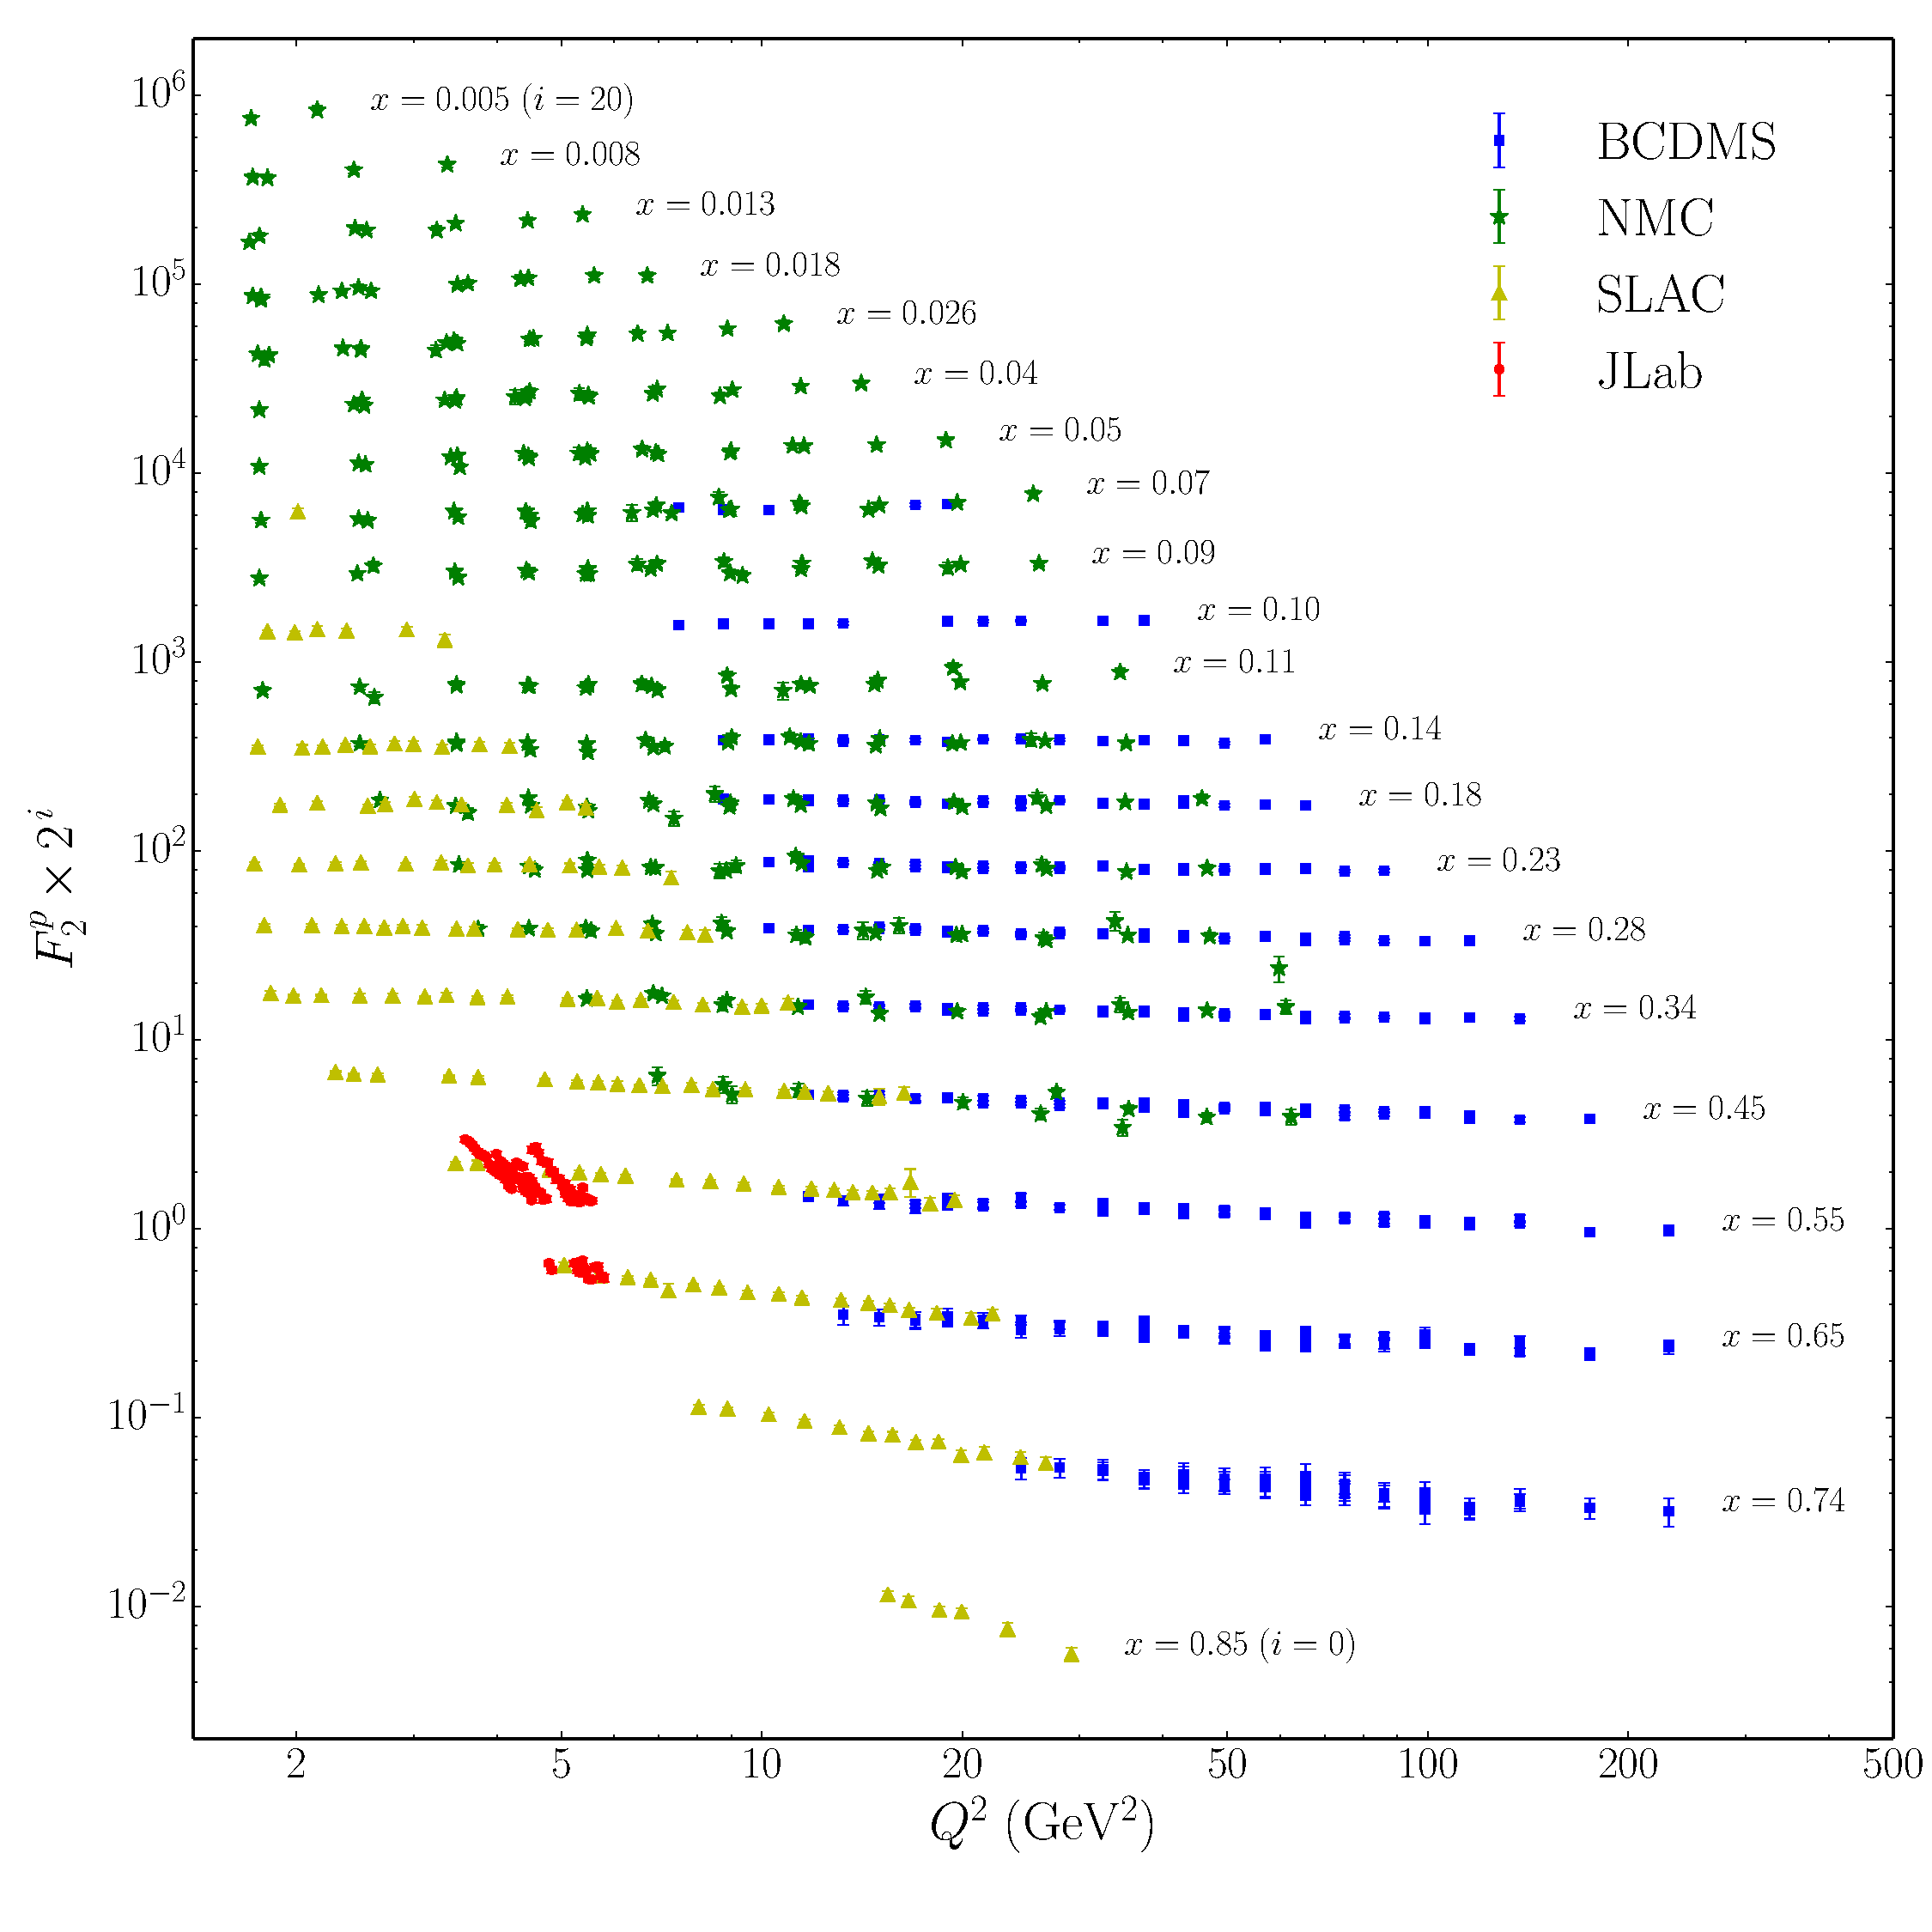
\includegraphics[width=15cm]{/u/group/cteqX/wmelnitc/CJgit/sharespace/codes/gallery/F2p.pdf}
\caption{Comparison of proton $F_2^p$ structure function data
	used in this analysis with the CJ15 fit.}
\label{fig:F2p}
\end{figure} 


\begin{figure}[t]
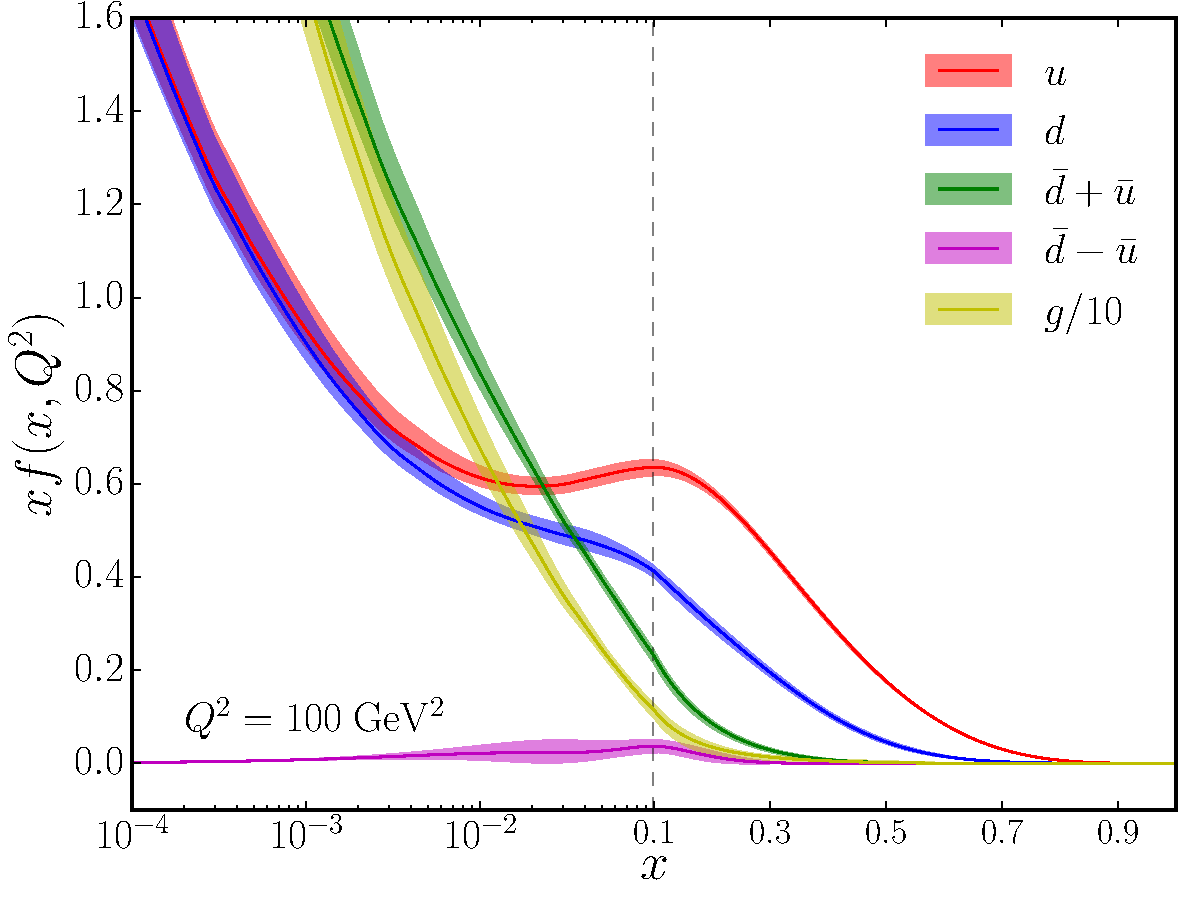
\includegraphics[width=12cm]{/u/group/cteqX/wmelnitc/CJgit/sharespace/codes/gallery/xpdf.pdf}
\caption{Comparison of CJ15 PDFs for different flavors
	($u, d, \bar d + \bar u, \bar d - \bar u$ and $g/10$)
	at a scale $Q^2=10$~GeV$^2$.
	Note the combined logarithim/linear scale along the $x$-axis.}
\label{fig:pdf}
\end{figure} 


\begin{figure}[t]
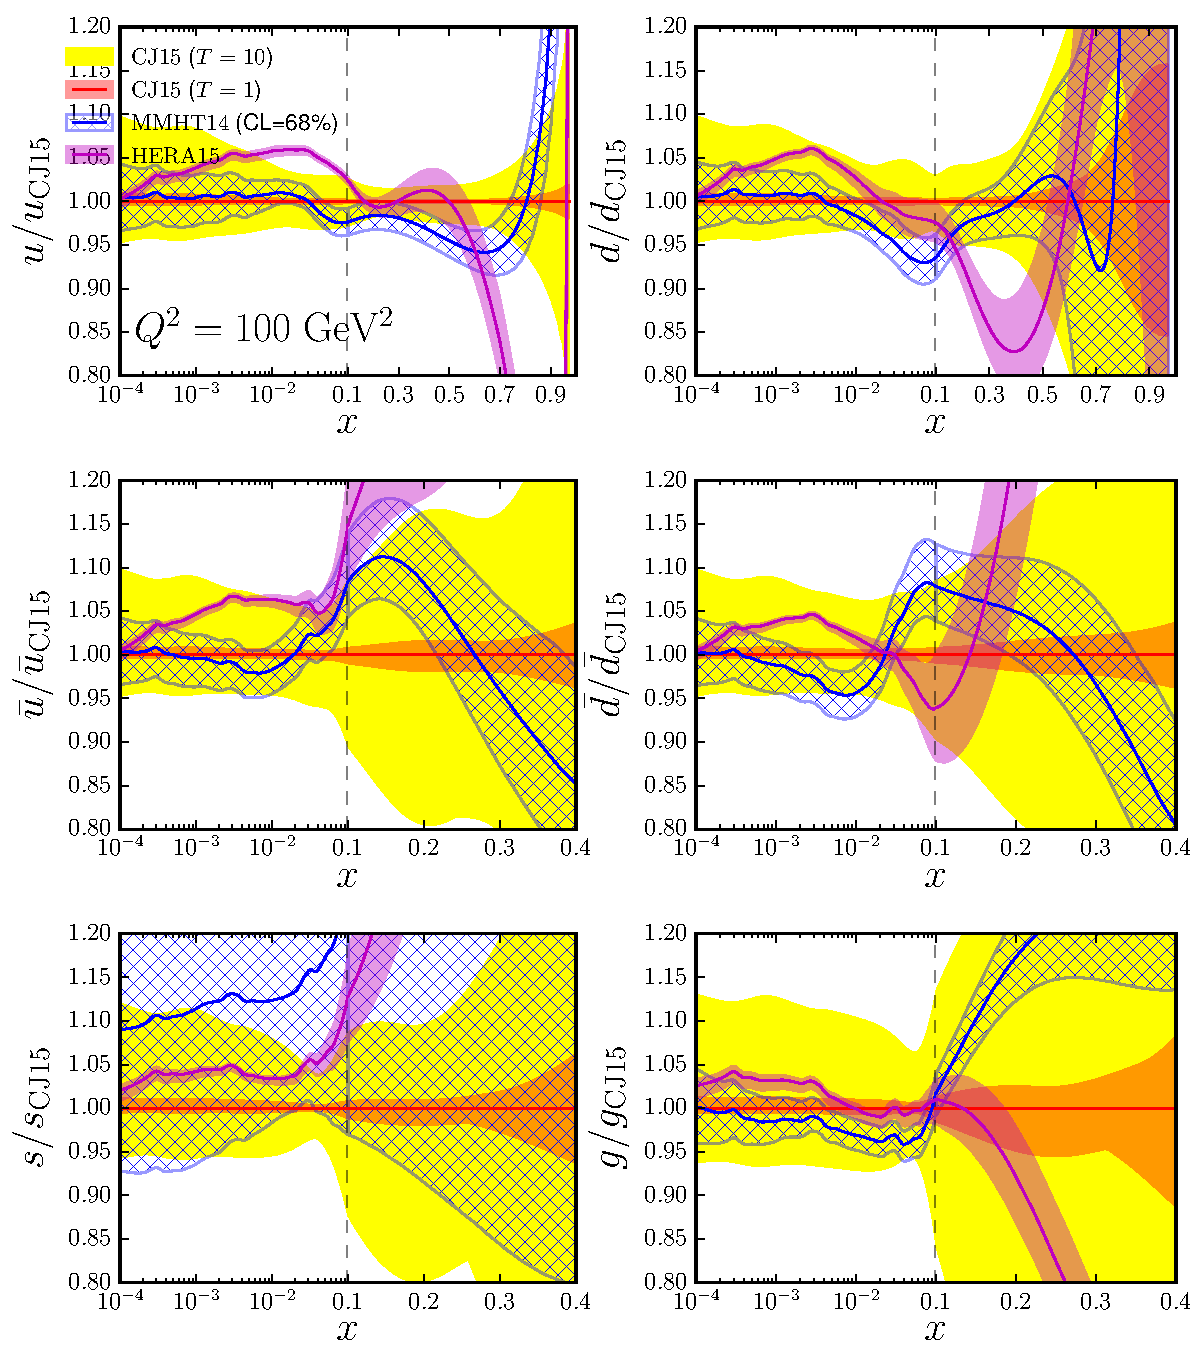
\includegraphics[width=15cm]{/u/group/cteqX/wmelnitc/CJgit/sharespace/codes/gallery/ratio.pdf}
\caption{Ratio of PDFs to the CJ15 central values for various PDF sets:
	CJ15 for tolerance $T=1$ (red) and $T=10$ (yellow),
	MMHT14 \cite{MMHT14} (blue), and
	HERA15 \cite{HERA15} (green).
	Note the different scales on the vertical axes used for
	different flavors.}
\label{fig:ratio_other}
\end{figure} 


\begin{figure}[t]
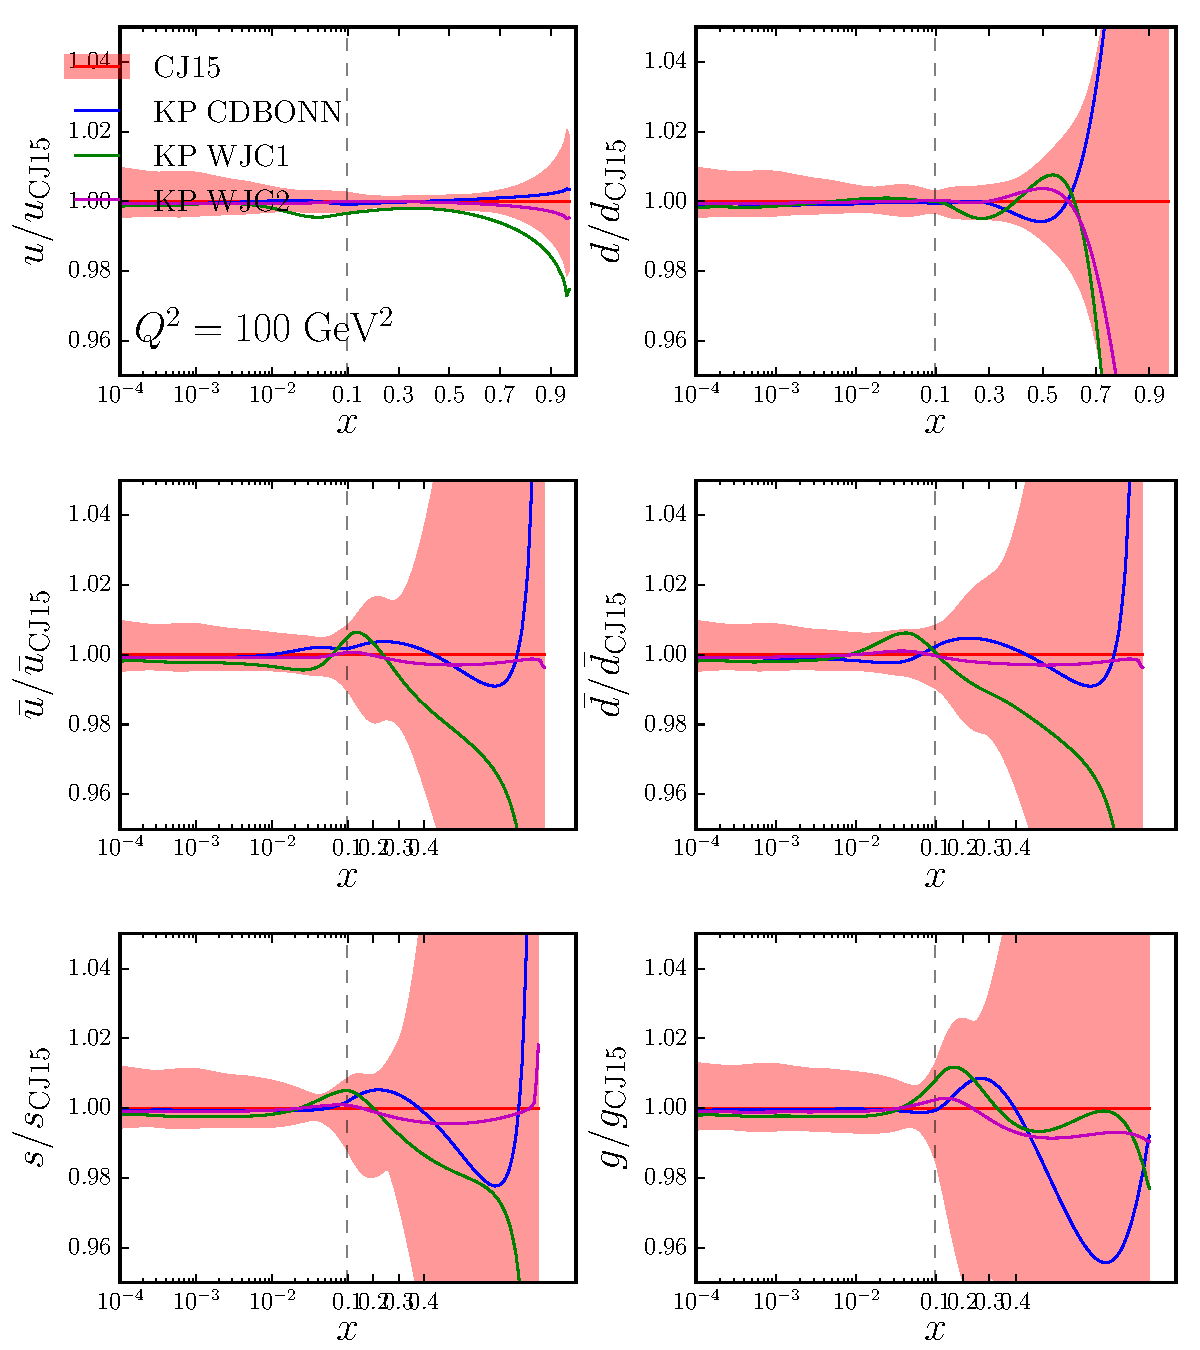
\includegraphics[width=15cm]{/u/group/cteqX/wmelnitc/CJgit/sharespace/codes/gallery/ratio_wfn.pdf}
\caption{Ratio of CJ15 PDFs (with $T=1$) for various deuteron
	wave function models:
	AV18 (yellow band),
	CD-Bonn (red solid lines),
	WJC-1 (green dashed lines),
	WJC-2 (blue solid lines),
	for the KP off-shell parametrization (\ref{eq:delffit}).
	The PDF ratios are taken with respect to those for the
	AV18 wave function.
	Note the different scale on the vertical axes for the
	$d$-quark and gluon distributions.}
\label{fig:ratio_wfn}
\end{figure} 


\begin{figure}[t]
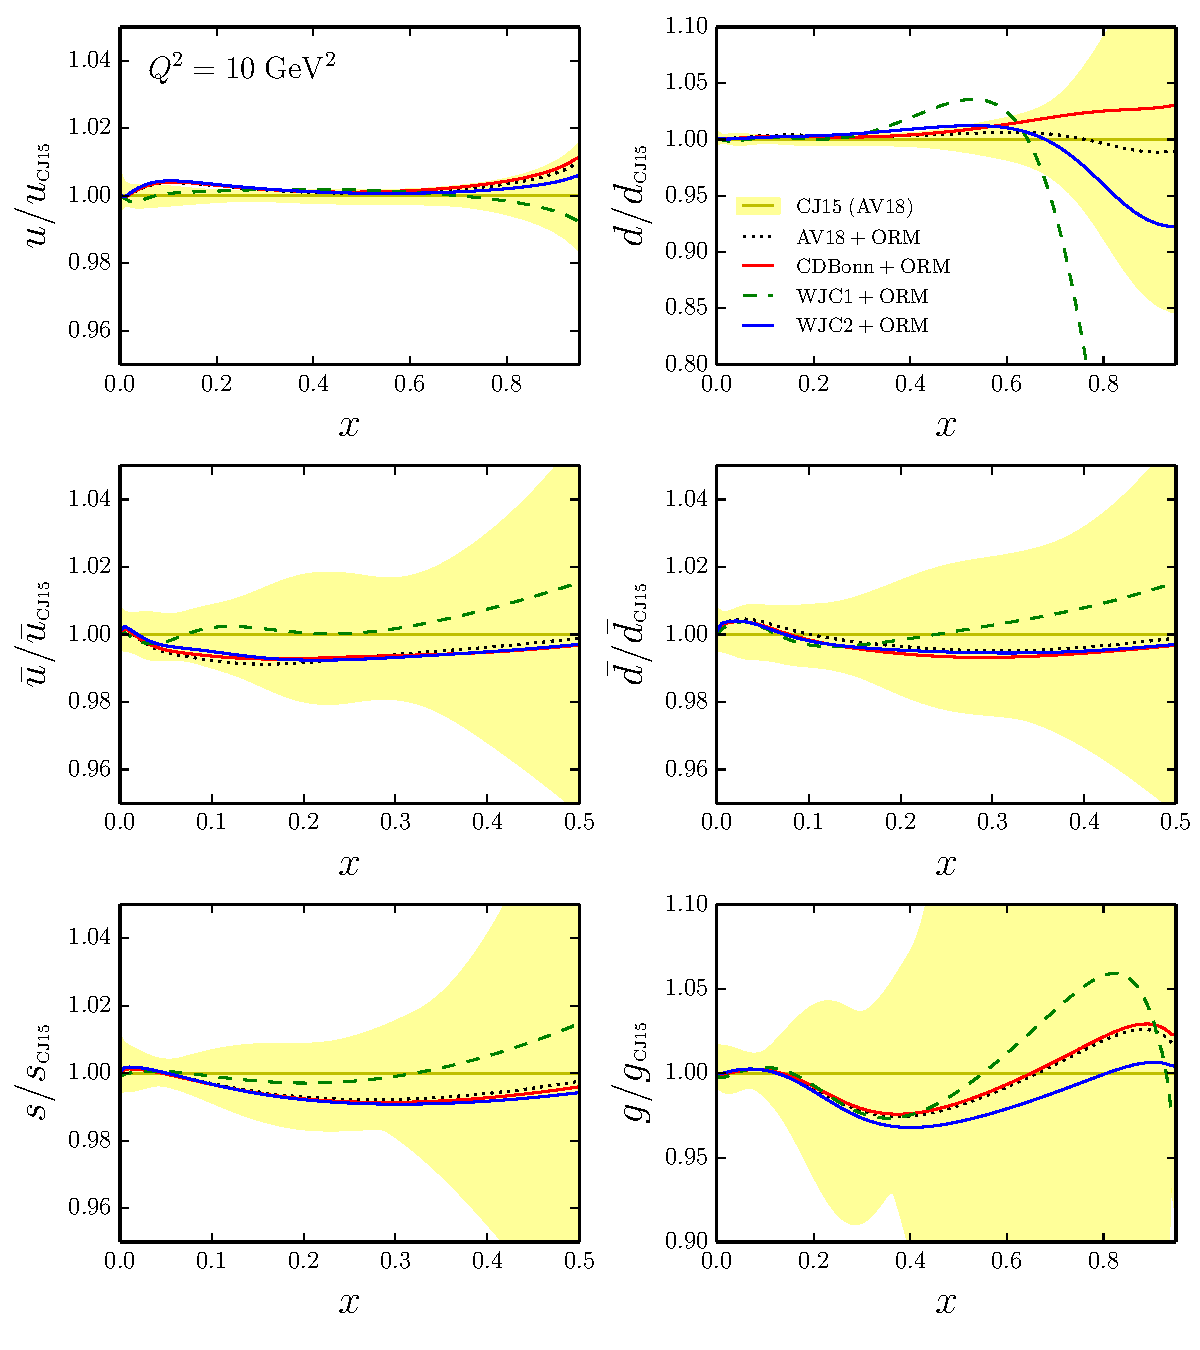
\includegraphics[width=15cm]{/u/group/cteqX/wmelnitc/CJgit/sharespace/codes/gallery/ratio_off.pdf}
\caption{Ratio of PDFs for the off-shell covariant spectator (OCS)
	model with different deuteron wave functions to the CJ15 PDFs
	(which uses the off-shell parametrization (\ref{eq:delffit})
	and the AV18 deuteron wave function):
	OCS model with AV18 (black dotted lines),
	CD-Bonn (red solid lines),
	WJC-1 (green dashed lines), and
	WJC-2 (blue solid lines).
	Note the different scale on the vertical axes for the
	$d$-quark and gluon distributions.
	...[CHANGE LABELS ``ORM'' $\to$ ``OCS'']...}
\label{fig:ratio_off}
\end{figure} 


% \begin{figure}[t]
% 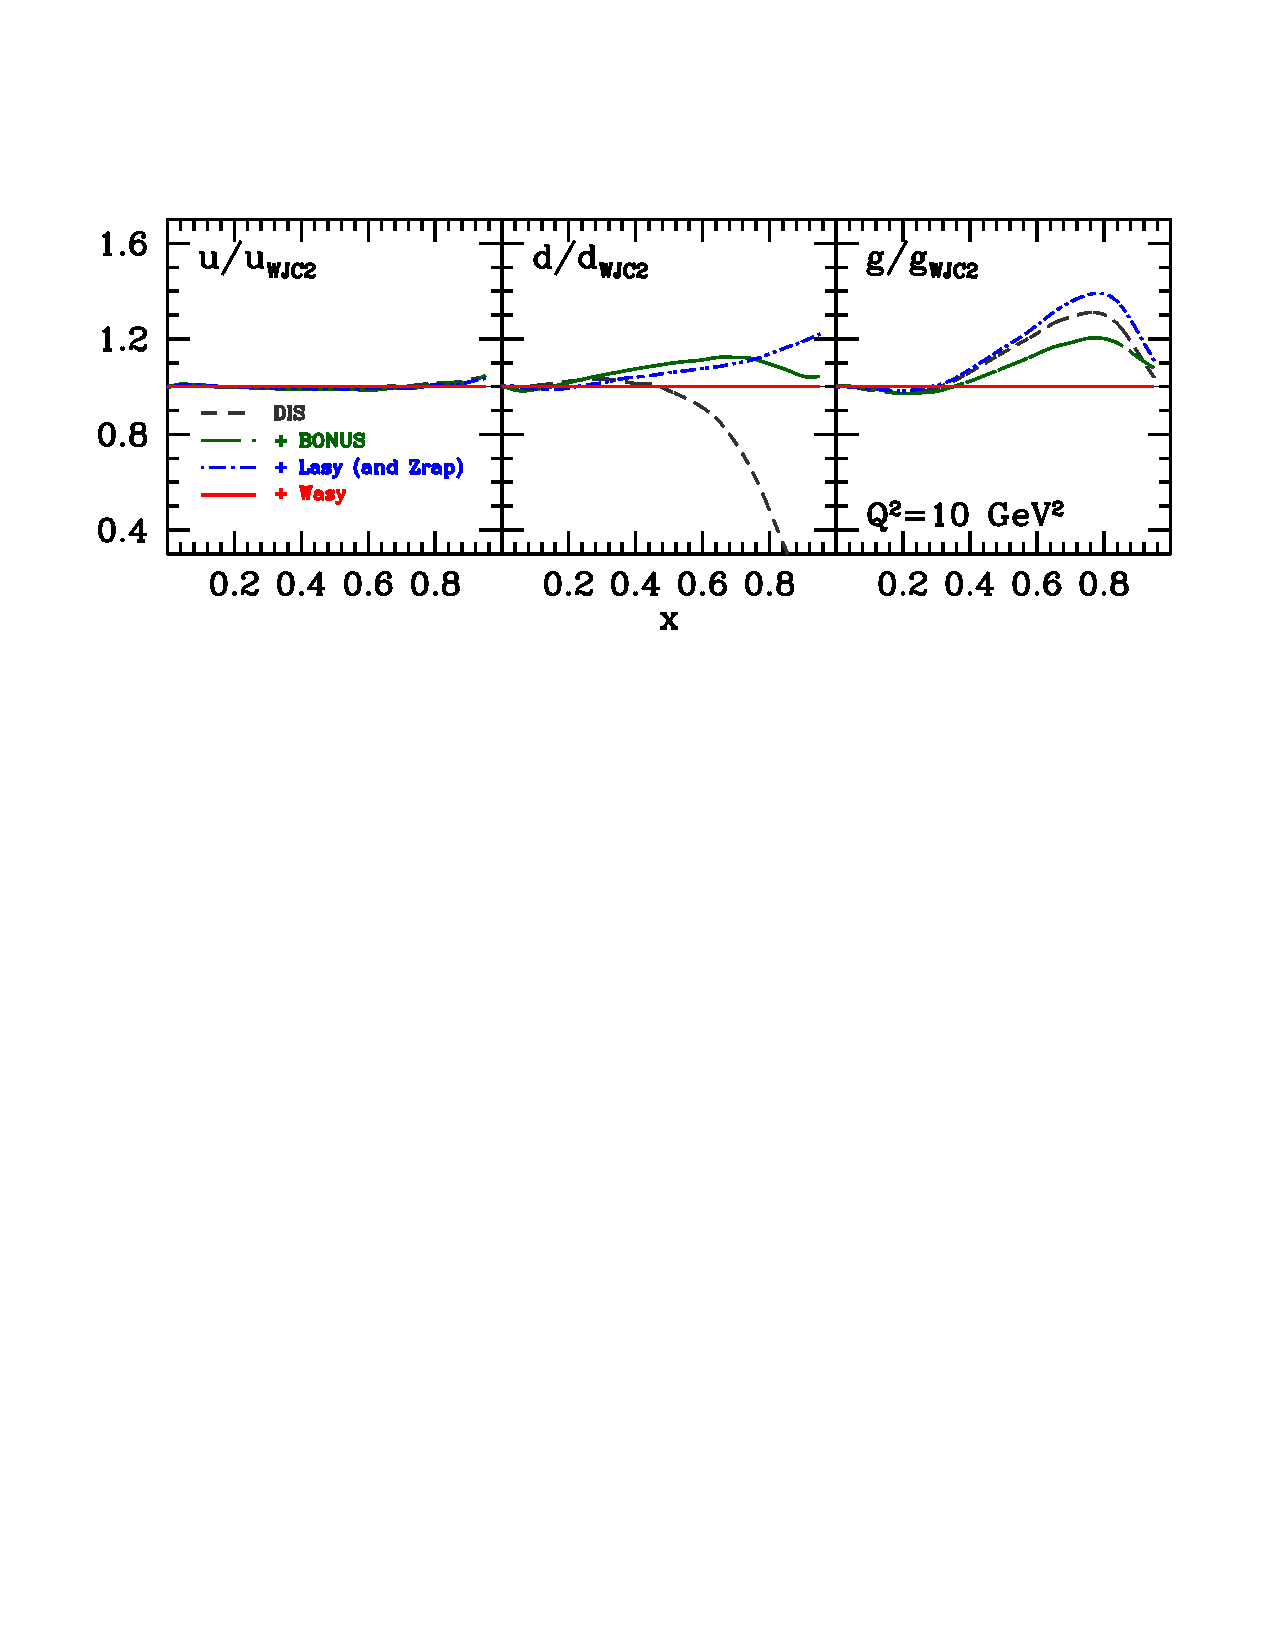
\includegraphics[width=15cm]{fig_BONUS_impact_pdfs.pdf}
% \vspace*{-12cm}
% \caption{Impact of BONuS \cite{BONuS} and $W$ asymmetry data
%	on the $u$, $d$ and $g$ distributions.}
% \label{fig:pdf_BONuS}
% \end{figure} 

  
% \begin{figure}[t]
% 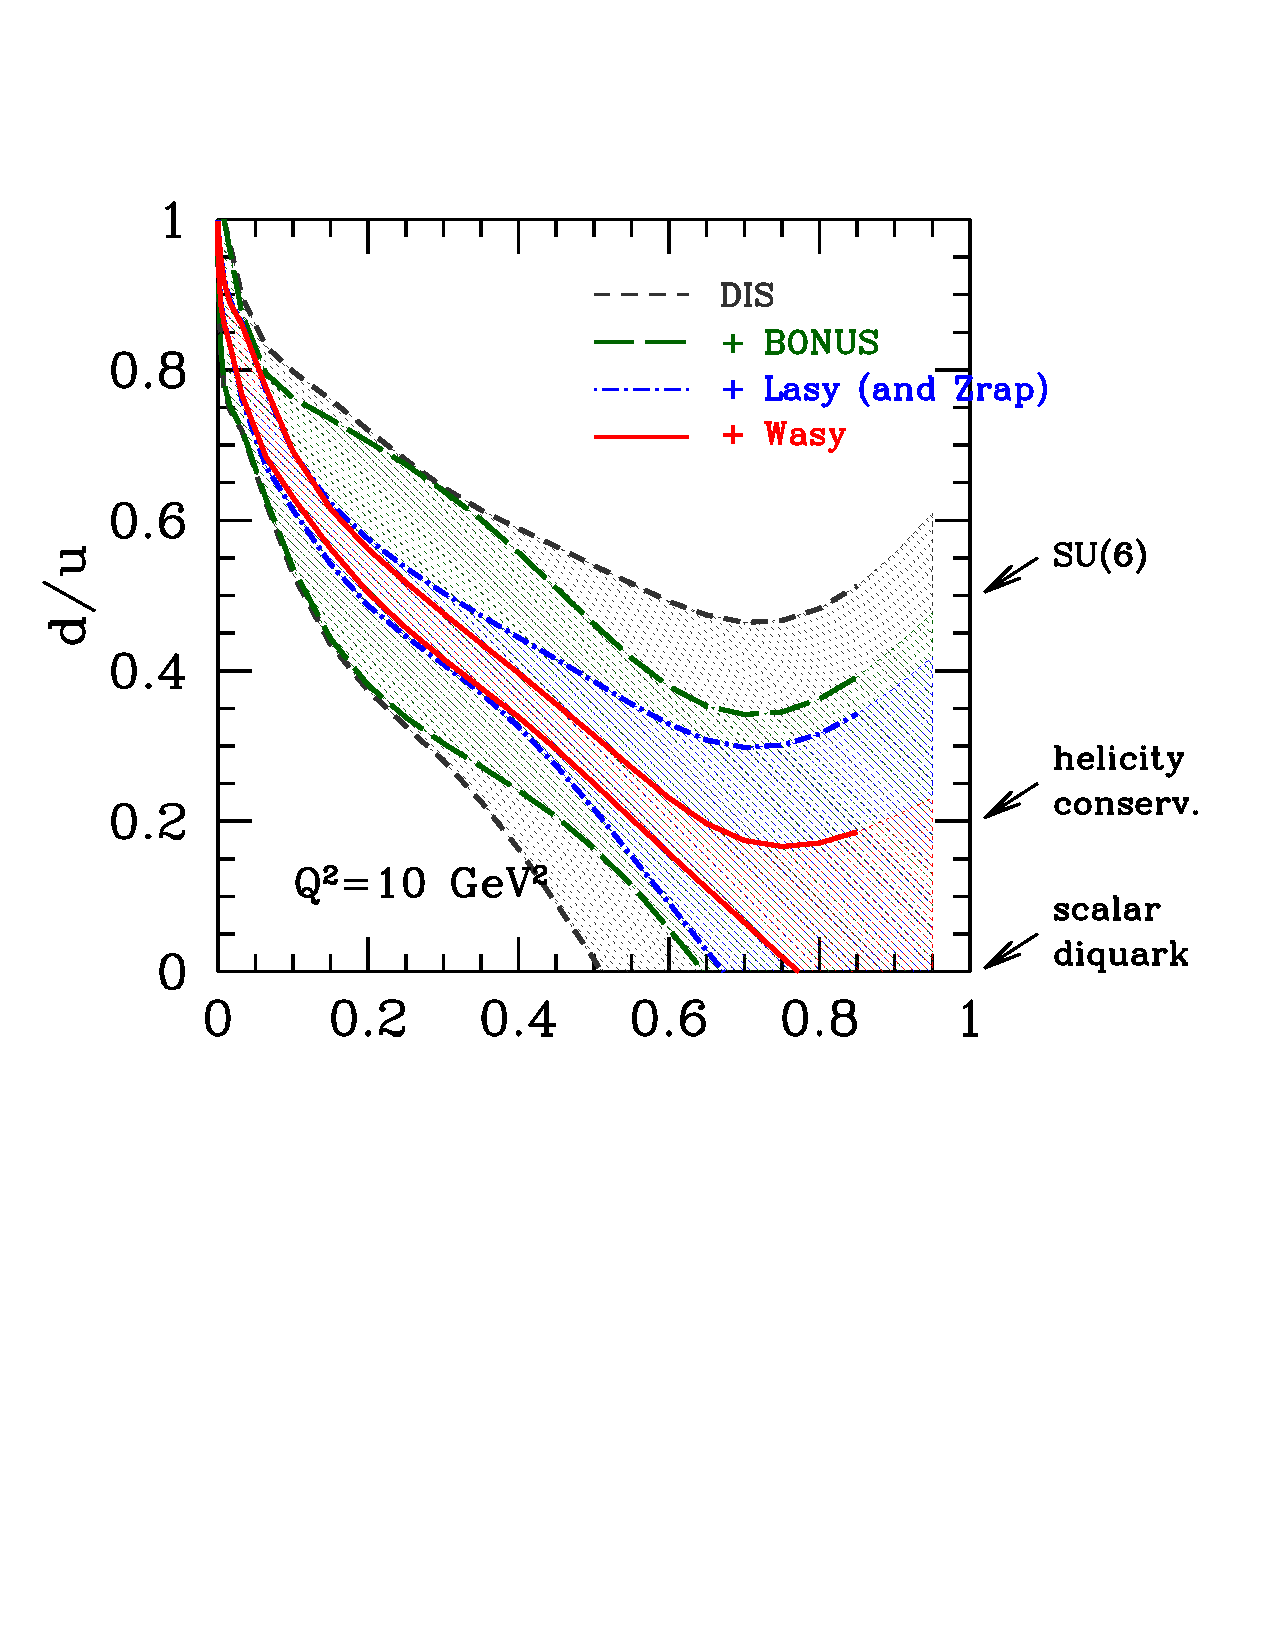
\includegraphics[width=12cm]{fig_BONUS_impact_du.pdf}
% \vspace*{-5cm}
% \caption{...[OLD FIGURE]...
%	Impact of BONuS \cite{BONuS} and $W$ asymmetry data
%	on the $d/u$ ratio.}
% \label{fig:du_BONuS}
% \end{figure} 


\begin{figure}[t]
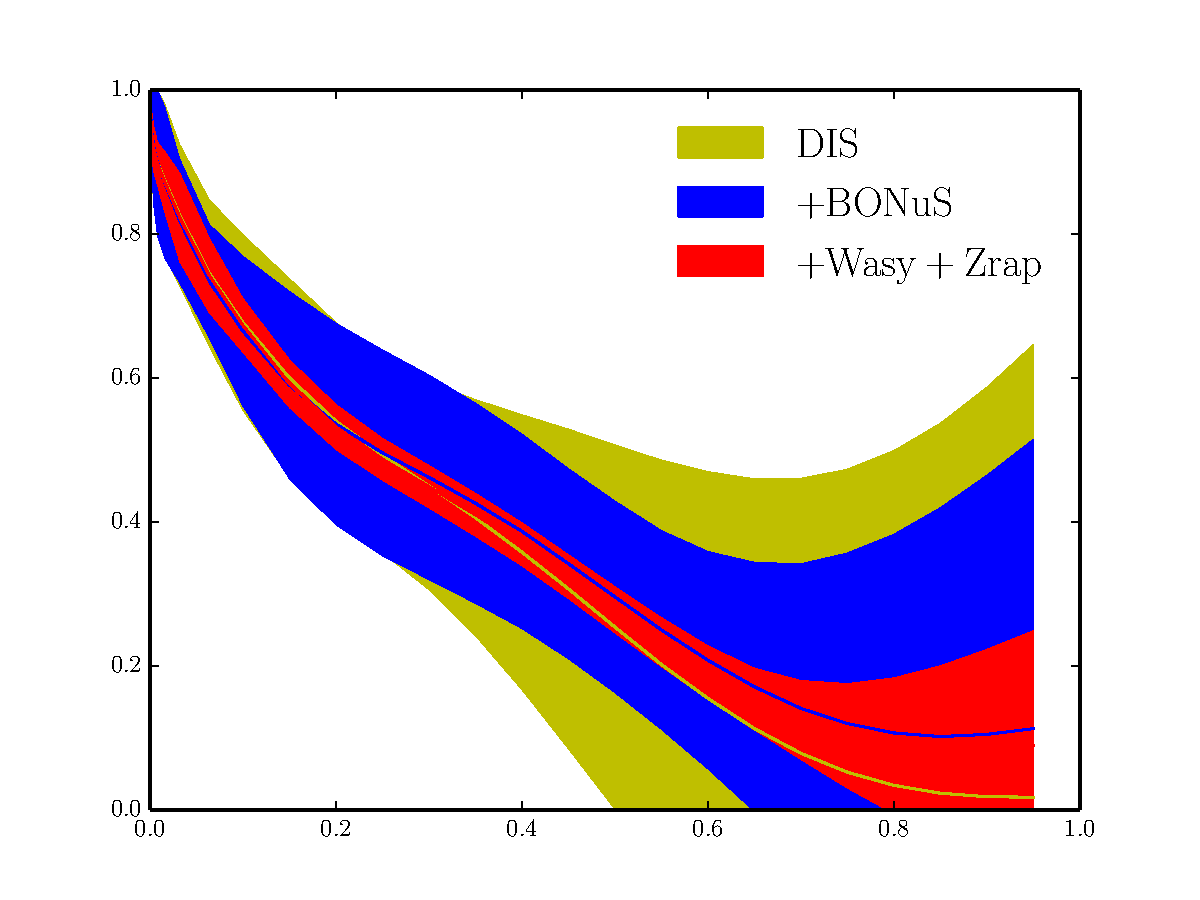
\includegraphics[width=12cm]{/u/group/cteqX/wmelnitc/CJgit/sharespace/codes/gallery/d_over_u.pdf}
\caption{Impact of BONuS \cite{BONuS} and $W$ asymmetry data
	on the $d/u$ ratio.}
\label{fig:du}
\end{figure} 


\begin{figure}[t]
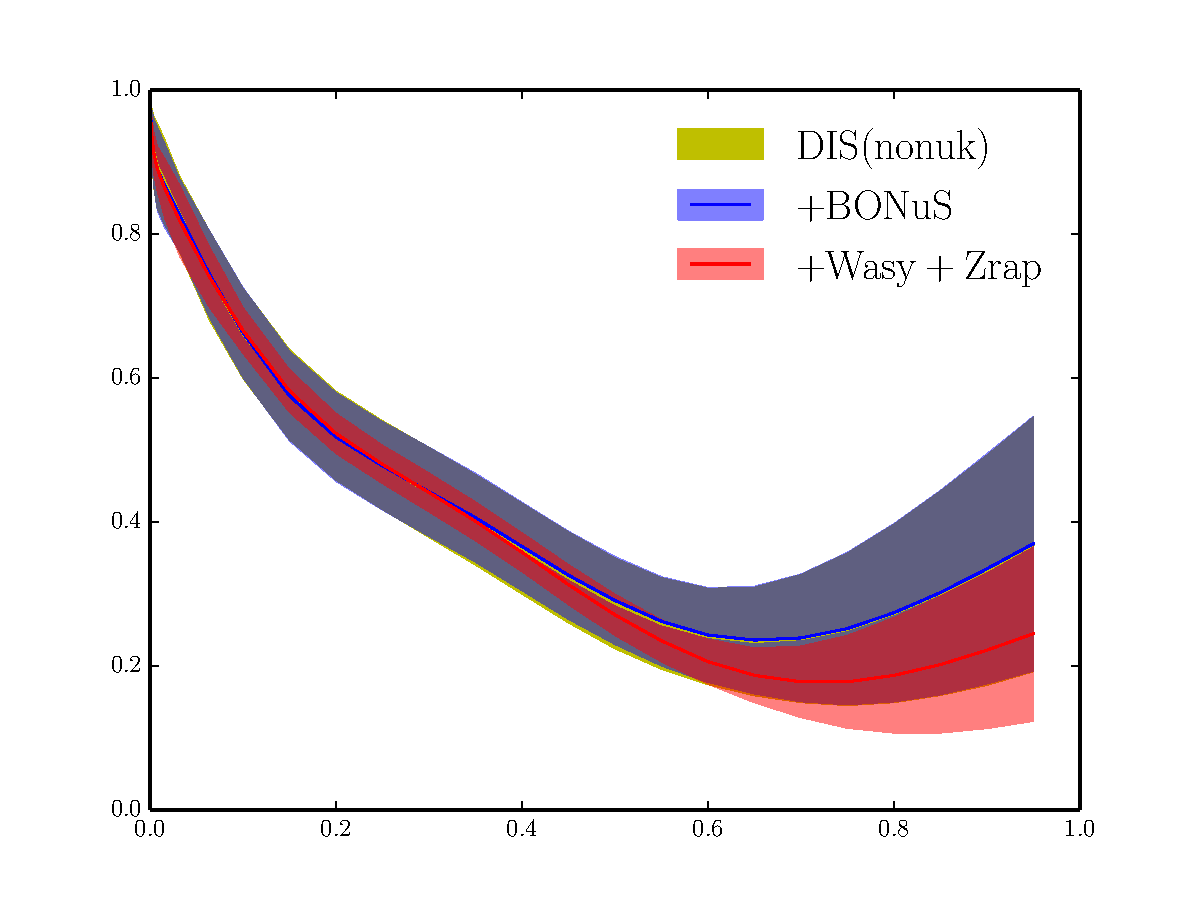
\includegraphics[width=12cm]{/u/group/cteqX/wmelnitc/CJgit/sharespace/codes/gallery/d_over_u1.pdf}
\caption{Impact of BONuS \cite{BONuS} and $W$ asymmetry data
	on the $d/u$ ratio, for the case of no nuclear corrections
	applied to the deuterium data.}
\label{fig:du1}
\end{figure} 


\end{document}


#########################################################################
#########################################################################
#########################################################################


% .......................................................................
\subsection{Theoretical errors}

...[OLD TEXT]

A significant source of theoretical errors is the modeling of nuclear
corrections for DIS on deuterium targets, which we refer to as
``nuclear uncertainty'' in short.  Of course, since the deuteron
can never be considered as composed of free nucleons, it is never
physically reasonable to assume no nuclear corrections at all.
We evaluate the nuclear uncertainty by considering nuclear corrections
ranging from mild, corresponding to the hardest of the modern deuteron
wave functions (WJC-1 \cite{WJC}) coupled to a 0.3\% nucleon swelling
effect, to strong, corresponding to the softest of the wave functions
(CD-Bonn \cite{CDBonn}) and a large, 2.1\% nucleon swelling.
An intermediate nuclear correction corresponding to the AV18
\cite{AV18} deuteron wave function and a 1.2\% nucleon swelling
effect is taken for our central fit.  These corrections approximately
span the same range as in our previous analysis \cite{CJ11}.


The effect of the different nuclear corrections is illustrated in
Fig.~\ref{fig:d2N} for the ratio of $F_2$ structure functions of the
deuteron and an idealized isoscalar target consisting of an unbound
proton and neutron.  The upper, middle, and lower curves are the
results for the mild (CJ12min), intermediate (CJ12mid), and strong
(CJ12max) nuclear corrections.  An intuitive way to understand the
effects of these nuclear corrections on global fits is to consider the
idealized free proton plus neutron target as being obtained by dividing
the deuterium target data by the ratio shown in Fig.~\ref{fig:d2N}.
In the intermediate-$x$ region the idealized nucleon $F_2^N$ structure
function is larger than the original data, and the increase is largest
for the maximum nuclear correction model.  On the other hand, as one
extends to values of $x$ above about 0.75, the reverse is true: the
$F_2^N$ results there lie below the data and are lowest for the mild
set of corrections. 


In a global fit, it is the combination of PDFs and nuclear corrections
which is constrained by deuterium data, not the PDFs alone.
At large $x$, the $u$ quark is well constrained by free proton DIS
and other data, so that when fitting the corrected deuterium data
(essentially the idealized $F_2^N \propto u+d$) the $d$ quark will
be the distribution most sensitive to the nuclear corrections.
Therefore, in the large-$x$ region the $d$ PDF will be smallest
for the mild correction and largest for the strong corrections
(see Fig.~\ref{fig:du} in Sec.~\ref{sec:results}).


One way to evaluate the impact of the nuclear uncertainty on a given
observable is by calculating it using the CJ12min fit corresponding
to the smallest nuclear correction, then with the CJ12max fit
corresponding to the largest correction. The values of the observable
spanning these 2 extremes can be considered a fair representation of
the theoretical nuclear uncertainty.  PDF errors can then be added
to the central values so calculated, and displayed as an outer error
band, as done in Ref.~\cite{CJ10, CJ11}.  Alternatively, one could first
calculate a PDF error band using the CJ12mid set, and display this on
top of the 2 bands obtained with the min and max sets.  The size of
the resulting sidebands will then represent the nuclear uncertainty.
